\documentclass[a4paper]{article}

\def\npart {III}
\def\nterm {Lent}
\def\nyear {2018}
\def\nlecturer {M.\ E.\ Cates}
\def\ncourse {Theoretical Physics of Soft Condensed Matter}
\def\ncoursehead {Soft Condensed Matter}

% Imports
\ifx \nextra \undefined
  \usepackage[pdftex,
    hidelinks,
    pdfauthor={Dexter Chua},
    pdfsubject={Cambridge Maths Notes: Part \npart\ - \ncourse},
    pdftitle={Part \npart\ - \ncourse},
  pdfkeywords={Cambridge Mathematics Maths Math \npart\ \nterm\ \nyear\ \ncourse}]{hyperref}
  \title{Part \npart\ - \ncourse}
\else
  \usepackage[pdftex,
    hidelinks,
    pdfauthor={Dexter Chua},
    pdfsubject={Cambridge Maths Notes: Part \npart\ - \ncourse\ (\nextra)},
    pdftitle={Part \npart\ - \ncourse\ (\nextra)},
  pdfkeywords={Cambridge Mathematics Maths Math \npart\ \nterm\ \nyear\ \ncourse\ \nextra}]{hyperref}

  \title{Part \npart\ - \ncourse \\ {\Large \nextra}}
\fi

\author{Lectured by \nlecturer \\\small Notes taken by Dexter Chua}
\date{\nterm\ \nyear}

\usepackage{alltt}
\usepackage{amsfonts}
\usepackage{amsmath}
\usepackage{amssymb}
\usepackage{amsthm}
\usepackage{booktabs}
\usepackage{caption}
\usepackage{enumitem}
\usepackage{fancyhdr}
\usepackage{graphicx}
\usepackage{mathtools}
\usepackage{microtype}
\usepackage{multirow}
\usepackage{pdflscape}
\usepackage{pgfplots}
\usepackage{siunitx}
\usepackage{tabularx}
\usepackage{tikz}
\usepackage{tkz-euclide}
\usepackage[normalem]{ulem}
\usepackage[all]{xy}

\pgfplotsset{compat=1.12}

\pagestyle{fancyplain}
\lhead{\emph{\nouppercase{\leftmark}}}
\ifx \nextra \undefined
  \rhead{
    \ifnum\thepage=1
    \else
      \npart\ \ncourse
    \fi}
\else
  \rhead{
    \ifnum\thepage=1
    \else
      \npart\ \ncourse\ (\nextra)
    \fi}
\fi
\usetikzlibrary{arrows}
\usetikzlibrary{decorations.markings}
\usetikzlibrary{decorations.pathmorphing}
\usetikzlibrary{positioning}
\usetikzlibrary{fadings}
\usetikzlibrary{intersections}
\usetikzlibrary{cd}

\newcommand*{\Cdot}{\raisebox{-0.25ex}{\scalebox{1.5}{$\cdot$}}}
\newcommand {\pd}[2][ ]{
  \ifx #1 { }
    \frac{\partial}{\partial #2}
  \else
    \frac{\partial^{#1}}{\partial #2^{#1}}
  \fi
}

% Theorems
\theoremstyle{definition}
\newtheorem*{aim}{Aim}
\newtheorem*{axiom}{Axiom}
\newtheorem*{claim}{Claim}
\newtheorem*{cor}{Corollary}
\newtheorem*{defi}{Definition}
\newtheorem*{eg}{Example}
\newtheorem*{fact}{Fact}
\newtheorem*{law}{Law}
\newtheorem*{lemma}{Lemma}
\newtheorem*{notation}{Notation}
\newtheorem*{prop}{Proposition}
\newtheorem*{thm}{Theorem}

\renewcommand{\labelitemi}{--}
\renewcommand{\labelitemii}{$\circ$}
\renewcommand{\labelenumi}{(\roman{*})}

\let\stdsection\section
\renewcommand\section{\newpage\stdsection}

% Strike through
\def\st{\bgroup \ULdepth=-.55ex \ULset}

% Maths symbols
\newcommand{\bra}{\langle}
\newcommand{\ket}{\rangle}

\newcommand{\N}{\mathbb{N}}
\newcommand{\Z}{\mathbb{Z}}
\newcommand{\Q}{\mathbb{Q}}
\renewcommand{\H}{\mathbb{H}}
\newcommand{\R}{\mathbb{R}}
\newcommand{\C}{\mathbb{C}}
\newcommand{\Prob}{\mathbb{P}}
\renewcommand{\P}{\mathbb{P}}
\newcommand{\E}{\mathbb{E}}
\newcommand{\F}{\mathbb{F}}
\newcommand{\cU}{\mathcal{U}}
\newcommand{\RP}{\mathbb{RP}}
\newcommand{\CP}{\mathbb{CP}}

\newcommand{\ph}{\,\cdot\,}

\DeclareMathOperator{\sech}{sech}
\DeclareMathOperator{\cosech}{cosech}
\DeclareMathOperator{\cosec}{cosec}

\DeclareMathOperator{\covol}{covol}
\DeclareMathOperator{\vol}{vol}

\let\Im\relax
\let\Re\relax
\DeclareMathOperator{\Im}{Im}
\DeclareMathOperator{\Re}{Re}
\DeclareMathOperator{\im}{im}
\DeclareMathOperator{\image}{image}
\DeclareMathOperator{\Ann}{Ann}

\DeclareMathOperator*{\res}{res}
\DeclareMathOperator{\Res}{Res}
\DeclareMathOperator{\Ind}{Ind}

\DeclareMathOperator{\tr}{tr}
\DeclareMathOperator{\diag}{diag}
\DeclareMathOperator{\rank}{rank}
\DeclareMathOperator{\card}{card}
\DeclareMathOperator{\spn}{span}
\DeclareMathOperator{\adj}{adj}

\DeclareMathOperator{\erf}{erf}
\DeclareMathOperator{\erfc}{erfc}

\DeclareMathOperator{\ord}{ord}
\DeclareMathOperator{\Sym}{Sym}

\DeclareMathOperator{\sgn}{sgn}
\DeclareMathOperator{\orb}{orb}
\DeclareMathOperator{\stab}{stab}
\DeclareMathOperator{\ccl}{ccl}

\DeclareMathOperator{\lcm}{lcm}
\DeclareMathOperator{\hcf}{hcf}

\DeclareMathOperator{\Int}{Int}
\DeclareMathOperator{\id}{id}

\DeclareMathOperator{\betaD}{beta}
\DeclareMathOperator{\gammaD}{gamma}
\DeclareMathOperator{\Poisson}{Poisson}
\DeclareMathOperator{\binomial}{binomial}
\DeclareMathOperator{\multinomial}{multinomial}
\DeclareMathOperator{\Bernoulli}{Bernoulli}
\DeclareMathOperator{\like}{like}

\DeclareMathOperator{\var}{var}
\DeclareMathOperator{\cov}{cov}
\DeclareMathOperator{\bias}{bias}
\DeclareMathOperator{\mse}{mse}
\DeclareMathOperator{\corr}{corr}

\DeclareMathOperator{\otp}{otp}
\DeclareMathOperator{\dom}{dom}

\DeclareMathOperator{\Root}{Root}
\DeclareMathOperator{\supp}{supp}
\DeclareMathOperator{\rel}{rel}
\DeclareMathOperator{\Hom}{Hom}
\DeclareMathOperator{\Aut}{Aut}
\DeclareMathOperator{\Gal}{Gal}
\DeclareMathOperator{\Mat}{Mat}
\DeclareMathOperator{\End}{End}
\DeclareMathOperator{\Char}{char}
\DeclareMathOperator{\ev}{ev}
\DeclareMathOperator{\St}{St}
\DeclareMathOperator{\Lk}{Lk}
\DeclareMathOperator{\disc}{disc}
\DeclareMathOperator{\Isom}{Isom}
\DeclareMathOperator{\length}{length}
\DeclareMathOperator{\energy}{energy}
\DeclareMathOperator{\area}{area}
\DeclareMathOperator{\Syl}{Syl}
\DeclareMathOperator{\cl}{cl}
\DeclareMathOperator{\fix}{fix}

\newcommand{\GL}{\mathrm{GL}}
\newcommand{\SL}{\mathrm{SL}}
\newcommand{\PGL}{\mathrm{PGL}}
\newcommand{\PSL}{\mathrm{PSL}}
\newcommand{\PSU}{\mathrm{PSU}}
\newcommand{\Or}{\mathrm{O}}
\newcommand{\SO}{\mathrm{SO}}
\newcommand{\U}{\mathrm{U}}
\newcommand{\SU}{\mathrm{SU}}

\renewcommand{\d}{\mathrm{d}}
\newcommand{\D}{\mathrm{D}}

\tikzset{->/.style = {decoration={markings,
                                  mark=at position 1 with {\arrow[scale=2]{latex'}}},
                      postaction={decorate}}}
\tikzset{<-/.style = {decoration={markings,
                                  mark=at position 0 with {\arrowreversed[scale=2]{latex'}}},
                      postaction={decorate}}}
\tikzset{<->/.style = {decoration={markings,
                                   mark=at position 0 with {\arrowreversed[scale=2]{latex'}},
                                   mark=at position 1 with {\arrow[scale=2]{latex'}}},
                       postaction={decorate}}}
\tikzset{->-/.style = {decoration={markings,
                                   mark=at position #1 with {\arrow[scale=2]{latex'}}},
                       postaction={decorate}}}
\tikzset{-<-/.style = {decoration={markings,
                                   mark=at position #1 with {\arrowreversed[scale=2]{latex'}}},
                       postaction={decorate}}}

\tikzset{circ/.style = {fill, circle, inner sep = 0, minimum size = 3}}
\tikzset{mstate/.style={circle, draw, blue, text=black, minimum width=0.7cm}}

\definecolor{mblue}{rgb}{0.2, 0.3, 0.8}
\definecolor{morange}{rgb}{1, 0.5, 0}
\definecolor{mgreen}{rgb}{0.1, 0.4, 0.2}
\definecolor{mred}{rgb}{0.5, 0, 0}

\def\drawcirculararc(#1,#2)(#3,#4)(#5,#6){%
    \pgfmathsetmacro\cA{(#1*#1+#2*#2-#3*#3-#4*#4)/2}%
    \pgfmathsetmacro\cB{(#1*#1+#2*#2-#5*#5-#6*#6)/2}%
    \pgfmathsetmacro\cy{(\cB*(#1-#3)-\cA*(#1-#5))/%
                        ((#2-#6)*(#1-#3)-(#2-#4)*(#1-#5))}%
    \pgfmathsetmacro\cx{(\cA-\cy*(#2-#4))/(#1-#3)}%
    \pgfmathsetmacro\cr{sqrt((#1-\cx)*(#1-\cx)+(#2-\cy)*(#2-\cy))}%
    \pgfmathsetmacro\cA{atan2(#2-\cy,#1-\cx)}%
    \pgfmathsetmacro\cB{atan2(#6-\cy,#5-\cx)}%
    \pgfmathparse{\cB<\cA}%
    \ifnum\pgfmathresult=1
        \pgfmathsetmacro\cB{\cB+360}%
    \fi
    \draw (#1,#2) arc (\cA:\cB:\cr);%
}
\newcommand\getCoord[3]{\newdimen{#1}\newdimen{#2}\pgfextractx{#1}{\pgfpointanchor{#3}{center}}\pgfextracty{#2}{\pgfpointanchor{#3}{center}}}

\def\Xint#1{\mathchoice
   {\XXint\displaystyle\textstyle{#1}}%
   {\XXint\textstyle\scriptstyle{#1}}%
   {\XXint\scriptstyle\scriptscriptstyle{#1}}%
   {\XXint\scriptscriptstyle\scriptscriptstyle{#1}}%
   \!\int}
\def\XXint#1#2#3{{\setbox0=\hbox{$#1{#2#3}{\int}$}
     \vcenter{\hbox{$#2#3$}}\kern-.5\wd0}}
\def\ddashint{\Xint=}
\def\dashint{\Xint-}

% lectures 19, 21, not 23, not 26, not 28, 2, 5, 7

\newcommand\splus{\!{\vphantom{\prod}}^+}
\begin{document}
\maketitle
{\small
\setlength{\parindent}{0em}
\setlength{\parskip}{1em}
Soft Condensed Matter refers to liquid crystals, emulsions, molten polymers and other microstructured fluids or semi-solid materials. Alongside many high-tech examples, domestic and biological instances include mayonnaise, toothpaste, engine oil, shaving cream, and the lubricant that stops our joints scraping together. Their behaviour is classical ($\hbar = 0$) but rarely is it deterministic: thermal noise is generally important.

The basic modelling approach therefore involves continuous classical field theories, generally with noise so that the equations of motion are stochastic PDEs. The form of these equations is helpfully constrained by the requirement that the Boltzmann distribution is regained in the steady state (when this indeed holds, i.e.\ for systems in contact with a heat bath but not subject to forcing). Both the dynamical and steady-state behaviours have a natural expression in terms of path integrals, defined as weighted sums of trajectories (for dynamics) or configurations (for steady state). These concepts will be introduced in a relatively informal way, focusing on how they can be used for actual calculations.

In many cases mean-field treatments are sufficient, simplifying matters considerably. But we will also meet examples such as the phase transition from an isotropic fluid to a `smectic liquid crystal' (a layered state which is periodic, with solid-like order, in one direction but can flow freely in the other two). Here mean-field theory gets the wrong answer for the order of the transition, but the right one is found in a self-consistent treatment that lies one step beyond mean-field (and several steps short of the renormalization group, whose application to classical
field theories is discussed in other courses but not this one).

Important models of soft matter include diffusive $\phi^4$ field theory (`Model B'), and the noisy Navier--Stokes equation which describes fluid mechanics at colloidal scales, where the noise term is responsible for Brownian motion of suspended particles in a fluid. Coupling these together creates `Model H', a theory that describes the physics of fluid-fluid mixtures (that is, emulsions). We will explore Model B, and then Model H, in some depth. We will also explore the continuum theory of nematic liquid crystals, which spontaneously break rotational but not translational symmetry, focusing on topological defects and their associated mathematical structure such as homotopy classes.

Finally, the course will cover some recent extensions of the same general approach to systems whose microscopic dynamics does not have time-reversal symmetry, such as self-propelled colloidal swimmers. These systems do not have a Boltzmann distribution in steady state; without that constraint, new field theories arise that are the subject of ongoing research.
\subsubsection*{Pre-requisites}
Knowledge of Statistical Mechanics at an undergraduate level is essential. This course complements the following Michaelmas Term courses although none are prerequisites: Statistical Field Theory; Biological Physics and Complex Fluids; Slow Viscous Flow; Quantum Field Theory.
}
\tableofcontents

\section{Introduction}
\subsection{A brief overview}
In the course, we are going to study soft condensed matter. We first look at different types of soft condensed matter and some examples:
\begin{center}
  \begin{tabular}{ccc}
    \toprule
    Type & low-tech & high-tech\\
    \midrule
    emulsions & mayonnaise & pharmaceuticals \\
    suspensions & toothpaste & paints and ceramics\\
    liquid crystals & wet soap & displays \\
    polymers & gum & plastics\\
    \bottomrule
  \end{tabular}
\end{center}
What makes these soft and condensed?
\begin{itemize}
  \item They have a \term{shear modulus} $G$ of $\sim 10^2$--$10^7$ Pascals, which is to be compared with steel, which have a shear modulus of $10^{10}$ Pascals.

  \item In most cases (except foams), the \term{bulk modulus} $K$ remains large, with order of magnitude $K \sim 10^{10}$ Pascal. As $K/G \to \infty$, this is the same as the object is incompressible. In other words, they are easy to change in shape, but not in volume.
\end{itemize}

In general, soft condensed matter have slow response to changing conditions. They exhibit \term{viscoelasticity}. This is best understood with a graph. Suppose we suddenly apply a force on the material:
\begin{center}
  \begin{tikzpicture}
    \draw [->] (0, 0) -- (5, 0) node [right] {$t$};
    \draw [->] (0, 0) -- (0, 4) node [pos=0.5, left] {$\sigma_0$};

    \draw [thick, mblue](0, 0) .. controls (0.1, 2) .. (0.3, 2) -- (5, 2);
    \draw (-0.05, 2) -- (0.05, 2);
  \end{tikzpicture}
\end{center}
The response is given by
\begin{center}
  \begin{tikzpicture}
    \draw [->] (0, 0) -- (5, 0) node [right] {$t$};
    \draw [->] (0, 0) -- (0, 4) node [pos=0.5, left] {$\sigma_0$};

    \draw [thick, mblue](0, 0) .. controls (0.1, 2) .. (0.3, 2) -- (5, 2);
    \draw (-0.05, 2) -- (0.05, 2);

    \draw [dashed, thick, mred](0, 0) .. controls (0.2, 1) .. (0.6, 1) -- (2, 1) .. controls (2.5, 1) .. (3, 1.5) -- (5, 3.5);

    \draw (-0.05, 1) node [left] {$\sigma_0/G$} -- (0.05, 1);
    \draw (2, -0.05) node [below] {$\tau$} -- (2, 0.05);

    \draw (4, 2.5) -- (4.5, 2.5) -- (4.5, 3) node [pos=0.5, right] {$\eta^{-1}$};
  \end{tikzpicture}
\end{center}
Here the slope of the RHS is $\eta^{-1}$, and $\eta \approx G_0 \tau$ is the viscosity. Note that the time scale for the change is of the order of a few seconds! The reason for this is large internal length scales.
\begin{center}
  \begin{tabular}{cc}
    \toprule
    Thing & Length scale \\
    \midrule
    Polymer & $\SI{100}{\nano\meter}$\\
    Colloids & $\sim\SI{1}{\micro\meter}$\\
    Liquid crystal domains & $\sim\SI{1}{\micro\meter}$\\
    \bottomrule
  \end{tabular}
\end{center}
These are all much much larger than the length scale of atoms.

How should we understand and model these systems? First of all, quantum fluctuations are negligible. The time scale $\tau_Q$ of quantum fluctuations is given by
\[
  \hbar \omega_Q = \frac{\hbar}{\tau_Q} \simeq k_B T.
\]
At room temperature, we find that $\tau_Q\sim 10^{-13}\SI{}{\second}$, which is much much smaller than soft matter time scales, which are of the order of seconds and minutes. So we might as well set $\hbar = 0$.

However, the course would be short if there were no fluctuations at all. The counterpart is that \emph{thermal} fluctuations do matter. These are major players in this course.

To give an example, suppose we have some hard, spherical colloids suspended in water, each of radius $a \simeq \SI{1}{\micro\meter}$. An important quantity that determines the behaviour of the colloid is the \emph{volume fraction}
\[
  \Phi = \frac{4}{3} \pi a^3 \frac{N}{V},
\]
where $N$ is the number of colloid particles.

Experimentally, we observe that when $\Phi < 0.49$, then this behaves like fluid, and the colloids are free to move around.
\begin{center}
  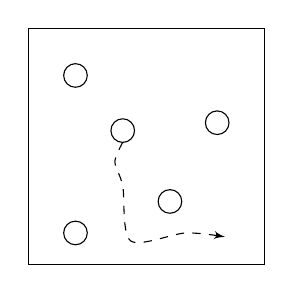
\begin{tikzpicture}
    \draw (0, 0) rectangle (3, 3);
    \draw (0.6, 0.4) circle [radius=0.15];
    \draw (1.8, 0.8) circle [radius=0.15];
    \draw (2.4, 1.8) circle [radius=0.15];
    \draw (0.6, 2.4) circle [radius=0.15];
    \draw (1.2, 1.7) circle [radius=0.15];
    \draw [-latex', dashed] plot [smooth] coordinates {(1.2, 1.55) (1.1, 1.3) (1.2, 1) (1.3, 0.3) (2, 0.4) (2.5, 0.35)};
  \end{tikzpicture}
\end{center}
In this regime, the colloid particles undergo Brownian motion, and we can ask how fast the particles move. It turns out The diffusivity constant is
\[
  D = \frac{k_B T}{6 \pi \eta_s a},
\]
where $\eta_s$ is the solvent viscosity. Thus, we can construct the timescale $\tau$ given by the time it takes to move through a distance of our own radius. In other words, we set $a^2 = D \tau$, and hence
\[
  \tau \sim \frac{a^3 \eta_s}{ k_B T}.
\]
When $\Phi > 0.55$, then the colloids fall into a crystal structure:
\begin{center}
  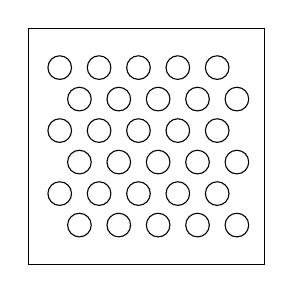
\begin{tikzpicture}
    \draw (-0.05, -0.1) rectangle +(3, 3);

    \draw (0.6, 0.4) circle [radius=0.15];
    \draw (1.1, 0.4) circle [radius=0.15];
    \draw (1.6, 0.4) circle [radius=0.15];
    \draw (2.1, 0.4) circle [radius=0.15];
    \draw (2.6, 0.4) circle [radius=0.15];

    \draw (0.35, 0.8) circle [radius=0.15];
    \draw (0.85, 0.8) circle [radius=0.15];
    \draw (1.35, 0.8) circle [radius=0.15];
    \draw (1.85, 0.8) circle [radius=0.15];
    \draw (2.35, 0.8) circle [radius=0.15];

    \draw (0.6, 1.2) circle [radius=0.15];
    \draw (1.1, 1.2) circle [radius=0.15];
    \draw (1.6, 1.2) circle [radius=0.15];
    \draw (2.1, 1.2) circle [radius=0.15];
    \draw (2.6, 1.2) circle [radius=0.15];

    \draw (0.35, 1.6) circle [radius=0.15];
    \draw (0.85, 1.6) circle [radius=0.15];
    \draw (1.35, 1.6) circle [radius=0.15];
    \draw (1.85, 1.6) circle [radius=0.15];
    \draw (2.35, 1.6) circle [radius=0.15];

    \draw (0.6, 2.0) circle [radius=0.15];
    \draw (1.1, 2.0) circle [radius=0.15];
    \draw (1.6, 2.0) circle [radius=0.15];
    \draw (2.1, 2.0) circle [radius=0.15];
    \draw (2.6, 2.0) circle [radius=0.15];

    \draw (0.35, 2.4) circle [radius=0.15];
    \draw (0.85, 2.4) circle [radius=0.15];
    \draw (1.35, 2.4) circle [radius=0.15];
    \draw (1.85, 2.4) circle [radius=0.15];
    \draw (2.35, 2.4) circle [radius=0.15];
  \end{tikzpicture}
\end{center}

Here the colloids don't necessarily touch, but there is still resistance to change in shape due to the entropy changes associated. We can find that the elasticity is given by
\[
  G \simeq k_B T \frac{N}{V}.
\]
In the small $\Phi$ case, the ``source'' of entropy is clear, given by the disorder in the position of the colloids. Here the entropy is given by the ``rattle room'' entropy.

In both cases, we see that the elasticity and time scales are given in terms of $k_B T$. If we ignore thermal fluctuations, then we have $G = 0$ and $\tau = \infty$, which is extremely boring, and more importantly, is not how the real world behaves!

\subsection{The general framework}
There are two parts to the study of soft condensed matters, confusingly and classically called \term{statics} and \term{dynamics}. The basic structure of the static part is going to look like this: we have some microscopic physics, but we don't want to track atoms and molecules. So we try to find some coarse-graining of the system. Thus, we come up with \emph{order parameter} fields, which we shall generically call $\psi(r)$. This goes into equilibrium statistical physics. To do this, we need to feed in symmetries and conservation laws. The output of this is some Boltzmann-distribution like probabilities $P[\psi(r)]$. In statistical physical field theory, $\psi$ might be our magnetization.

To do dynamics, we want to think of $\psi(r)$ as a function of space and time. The starting point is ``hydrodynamic'' PDEs of the form
\[
  \dot{\psi}(r, t) = \cdots,
\]
and the thing on the right hand side will depend on the type of substance we are talking about, and this is often informed by the static equilibrium statistical physics. The next step to realize is that even in dynamics, we cannot forget about thermal fluctuations. However, the PDE itself is deterministic. Thus, we have to promote these to stochastic PDEs, which are of the form
\[
  \dot{\psi}(r, t) = \cdots + \text{noise}.
\]
This is informed by the static probability given by the fluctuation dissipation theorem, which fixes the noise by requiring that it produces the right equilibrium statistics. If we have a stochastic equation like this, the basic thing we are trying to find out is the probability $\P[\psi(r, t)]$ of a certain evolution of a system, not only in space but also in time.

\begin{center}
  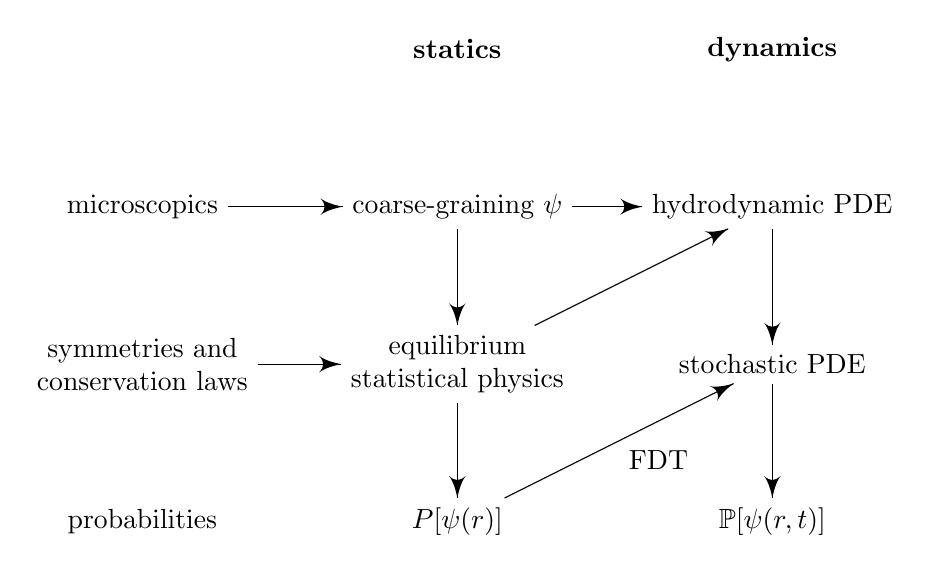
\begin{tikzpicture}[xscale=4, yscale=2]
    \node at (0, 0) {\textbf{statics}};
    \node at (1, 0) {\textbf{dynamics}};
    \node (mic) at (-1, -1) {microscopics};
    \node (coarse) at (0, -1) {coarse-graining $\psi$};
    \node (pde) at (1, -1) {hydrodynamic PDE};
    \node (sym) [align=center] at (-1, -2) {symmetries and\\ conservation laws};
    \node (equil) [align=center] at (0, -2) {equilibrium\\statistical physics};
    \node (stochastic) at (1, -2) {stochastic PDE};
    \node at (-1, -3) {probabilities};
    \node (p1) at (0, -3) {$P[\psi(r)]$};
    \node (p2) at (1, -3) {$\P[\psi(r, t)]$};

    \draw [->] (mic) -- (coarse);
    \draw [->] (sym) -- (equil);
    \draw [->] (coarse) -- (equil);
    \draw [->] (equil) -- (p1);
    \draw [->] (coarse) -- (pde);
    \draw [->] (pde) -- (stochastic);
    \draw [->] (equil) -- (pde);
    \draw [->] (p1) -- (stochastic) node [pos=0.5, anchor=north west] {FDT};
    \draw [->] (stochastic) -- (p2);
  \end{tikzpicture}
\end{center}
\begin{eg}
  $\psi(r, t)$ can consist of the density $\rho$ and velocity $\mathbf{v}$, and this describes a $1$-component isothermal fluid, e.g.\ water. The hydrodynamic PDE is exactly the fluid equations of motion.

  If we add a further composition function $\phi$, this describes a $2$-component fluid mixture. If we think about liquid crystals, then we need to add the molecular orientation. This actually requires a second-rank tensor $Q$, which describes a nematic liquid crystal.

  In the case of magnetism, we can add the magnetization $m$, but we will not do this in the course.
\end{eg}

\begin{eg}
  Consider isothermal, incompressible one-component fluid. The incompressibility condition is a simplification that lets us fix $\dot{\rho} = 0$. It follows that $\nabla \cdot \mathbf{v} = 0$. Then the equation in question is
  \[
    \rho (\dot{\mathbf{v}} + \mathbf{v} \cdot \nabla \mathbf{v}) = \eta \nabla^2 \mathbf{v} - \nabla p,
  \]
  the \term{Navier--Stokes equation}.

  We now promote this to a stochastic PDE. This is usually called the \term{Navier--Stokes--Landau--Lipschitz equation}, and is given by
  \[
    \rho (\dot{\mathbf{v}} + \mathbf{v} \cdot \nabla \mathbf{v}) = \eta \nabla^2 \mathbf{v} - \nabla p + \nabla \cdot \Sigma^N,
  \]
  The last term is thought of as a noise stress tensor on our fluid, and is conventionally treated as a Gaussian, and this is fixed by the fluctuation-dissipation theorem, and is given by
  \[
    \bra \Sigma_{ij}^N(r, t) \Sigma_{k \ell}^N (r', t')\ket = 2k_B T \eta (\delta_{i\ell} \delta_{jk} + \delta_{ik} \delta_{j\ell}) \delta(\mathbf{r} - \mathbf{r}') \delta(t - t').
  \]
\end{eg}

\section{Revision of equilibrium statistical physics}
\subsection{Thermodynamics}
The fastest route to getting the results we want is via Gibbs entropy.
\begin{defi}[Entropy]\index{entropy}
  The \emph{entropy} of a system is
  \[
    S = - k_B \sum_i p_i \log p_i,
  \]
  where $k_B$ is \term{Boltzmann's constant}, $i$ is a \term{microstate} --- a complete specification of the microscopics (e.g.\ the list of all particle coordinates and velocities) --- and $p_i$ is the probability of being in a certain microstate.
\end{defi}

The axiom of Gibbs is that a system in thermal equilibrium maximizes $S$ subject to applicable constraints.
\begin{eg}
  In an isolated system, which has a fixed number $N$ of particles, and fixed energy $E$ and volume $V$. We now want to maximize $S$ subject to the only constraint
  \[
    \sum_i p_i = 1.
  \]
  Writing $\lambda$ for the Lagrange multiplier maintaining this constraint, we require
  \[
    \frac{\partial}{\partial p_i} \left(S - \lambda \sum_i p_i\right) = 0.
  \]
  So we find that
  \[
    -k_B \log p_i + 1 - \lambda = 0
  \]
  for all $i$. In particular, all $p_i$ must be equal. Note that the sum is restricted to the states with the prescribed $N, E, V$. This is not the Boltzmann distribution, since we have completely isolated our system.
\end{eg}

\begin{eg}
  Consider a system of fixed contents ($N$) and volume $V$ in contact with a heat bath. So $E$ is no longer fixed, and fluctuates around some average $\bra E \ket = \bar{E}$. So we can apply Gibbs' principle again, where we now sum over all states of all $E$, with the restrictions
  \[
    \sum p_i E_i = \bar{E},\quad \sum p_i = 1.
  \]
  So our equation is
  \[
    \frac{\partial}{\partial p_i} \left(S - \lambda_I \sum p_i - \lambda_E \sum p_i E_i\right) = 0.
  \]
  Differentiating this with respect to $p_i$, we get
  \[
     -k_B (\log p_i + 1) - \lambda_I - \lambda_E E_i = 0.
  \]
  So it follows that
  \[
    p_i = \frac{1}{Z} e^{-\beta E_i},
  \]
  where $Z = \sum_i e^{-\beta E_i}$ and $\beta = \lambda_E/k_B$. This is the Boltzmann distribution.

  What is this mysterious $\beta$? Recall that the Lagrange multiplier $\lambda_E$ measures how $S$ reacts to a change in $\bar{E}$. In other words,
   \[
    \frac{\partial S}{\partial E} = \lambda_E = \kappa_B \beta.
  \]
  Moreover, \emph{by definition} of temperature\index{temperature}, we have
  \[
    \left.\frac{\partial S}{\partial E}\right|_{V, N, \ldots} = \frac{1}{T}.
  \]
j So it follows that
  \[
    \beta = \frac{1}{k_B T}.
  \]
\end{eg}
Recall that the first law of thermodynamics says
\[
  \d E = T\;\d S - P \;\d V + \mu \;\d N + \cdots.
\]
This is a natural object to deal with when we have fixed $S, V, N$, etc. However, often, it is temperature that is fixed, and it is more natural to consider the free energy:
\begin{defi}[Helmholtz free energy]\index{Helmholtz free energy}
  The \emph{Helmholtz free energy} of a system at fixed temperature, volume and particle number is defined by
  \[
    F(T, V, N) = U - TS = \bar{E} - TS = - k_B T \log Z.
  \]
\end{defi}
This satisfies
\[
  \d F = -S \;\d T - P\;\d V + \mu\;\d N + \cdots,
\]
and is minimized at equilibrium for fixed $T, V, N$. The derivative of $F$ in an isothermal system tells us ``which way it moves''.

\subsection{Coarse Graining}
Usually, in statistical mechanics, we distinguish between two types of objects --- microstates, namely the exact configuration of the system, and macrostates, which are variables that describe the overall behaviour of the system, such that pressure and temperature. Here we would like to consider something in between.

For example, if we have a system of magnets as in the Ising model, we the microstate would be the magnetization at each site, and the macrostate would be the overall magnetization. A coarse-graining of this would be a function $m(\mathbf{r})$ of space that describes the ``average magnetization around $\mathbf{r}$''. There is no fixed prescription on how large an area we average over, and usually it does not matter much.

In general, the coarse-grained variable would be called $\psi$. We can define a coarse-grained partition function
\[
  Z[\psi(\mathbf{r})] = \sum_{i \in \psi} e^{-\beta E_i},
\]
where we sum over all states that coarse-grain to $\psi$. We can similarly define the energy and entropy by restricting to all such $\psi$, and get
\[
  F[\psi] = E[\psi] - T S[\psi].
\]
The probability of being in a state $\psi$ is then
\[
  \P[\psi] = \frac{e^{-\beta F[\psi]}}{Z_{TOT}},\quad Z_{TOT} = \int e^{-\beta F[\psi]} \;\D [\psi].
\]
What we have on the end is a \emph{functional integral}, where we integrate over all possible values of $\psi$. We shall go into details later. We then have
\[
  F_{TOT} = -k_B T \log Z_{TOT}.
\]
In theory, one can obtain $F[\psi]$ by explicitly doing a coarse graining of the macroscopic laws. However, what is more common is to take a phenomenological approach, which is to figure out a $F[\psi]$ empirically.

We first give an example of explicit coarse graining.
\begin{eg}
  Consider an ideal gas with $N$ particles.
\end{eg}
% something

\section{Mean field theory}
\subsection{Binary fluids}
Consider a binary fluid, consisting of a mixture of two fluids $A$ and $B$. For simplicity, we assume we are in the symmetric case, where $A$ and $B$ are the same ``type'' of fluids. In other words, the potentials between the fluids are such that
\[
  U_{AA}(\mathbf{r}) = U_{BB}(\mathbf{r}) \not= U_{AB}(\mathbf{r}).
\]
We consider the case where $A$ and $B$ repulse each other (or rather, repulse each other more than the $A$-$A$ and $B$-$B$ repulsions). Thus, we expect that at high temperatures, entropy dominates, and the two fluids are mixed together well. At low temperatures, energy dominates, and the two fluids would be well-separated.

We let $\rho_A(\mathbf{r})$ and $\rho_B(\mathbf{r})$ be the coarse-grained particle density of each fluid, and we set our order parameter to be
\[
  \phi(\mathbf{r}) = \frac{\rho_A(\mathbf{r}) - \rho_B(\mathbf{r})}{(N_A + N_B)/V},
\]
with $N_A$ and $N_B$, the total amount of fluids $A$ and $B$, and $V$ the volume. This is normalized so that $\phi(\mathbf{r}) \in [-1, 1]$.

We model our system with \term{Landau--Ginzburg theory}, with free energy given by
\[
  \beta F = \int \Big(\underbrace{\frac{a}{2} \phi^2 + \frac{b}{4} \phi^4}_{f(\phi)} + \frac{\kappa}{2} (\nabla \phi)^2\Big)\;\d x,
\]
where $a, b, \kappa$ are functions of temperature.

Why did we pick such a model? Symmetry suggests the free energy should be even, and if we Taylor expand any even free energy functional, the first few terms will be of this form. For small $\phi$ and certain values of $a, b, \kappa$, we shall see there is no need to look further into higher order terms.

Observe that even without symmetry, we can always assume we do not have a linear term, since a $c \phi$ term will integrate out to give $cV \bar{\phi}$, and $\bar{\phi}$, the average composition of the fluid, is a fixed number. So this just leads to a constant shift.

The role of the gradient term $\int \frac{\kappa}{2} (\nabla \phi)^2 \;\d \mathbf{r}$ captures at order $\nabla^{(2)}$ the non-locality of $E_{int}$,
\[
  E_{int} = \int \rho_i (\mathbf{r}) \rho_j(\mathbf{r}') U_{ij}(|\mathbf{r} - \mathbf{r}'|)\;\d \mathbf{r}\;\d \mathbf{r}',
\]
where $i, j \in A, B$. If we assume $\phi(\mathbf{r})$ is slowly varying on the scale of interactions, then we can Taylor expand this $E_{int}$ and obtain a $(\nabla \phi)^2$ term.

What does this do to our system? The parameter $\kappa$ fixes the \term{interfacial tension},
\[
  \sigma = \left(\frac{-9 \kappa a^3}{9 b^2}\right)^{1/2}.
\]
See questions 6, 7 on the example sheet for more.

For this model to make sense, we want the free energy to be suppressed for large fluctuating $\phi$. Thus, we want $b, \kappa > 0$, while $a$ can take either sign. In general, the sign of $a$ is what determines the behaviour of the system, so for simplicity, we suppose $b$ and $\kappa$ are fixed, and let $a$ vary with temperature.

We now attempt to understand this with mean field theory. This means we look for a single $\phi(\mathbf{r})$ that minimizes $F$ (i.e.\ maximizes $P \propto e^{-\beta F}$).

Since the gradient term $\int \frac{\kappa}{2} (\nabla \phi)^2\;\d x \geq 0$, a naive guess would be that we should pick a uniform $\phi$,
\[
  \phi(\mathbf{r}) = \bar{\phi}.
\]
Note that $\bar{\phi}$ is fixed by the constraint of the system, namely how much fluid of each type we have. So we do not have any choice. We can write our free energy per unit volume as
\[
  \frac{F}{V} = f(\bar{\phi}) = \frac{a}{2} \bar{\phi}^2 + \frac{b}{4} \bar{\phi}^4.
\]
The behaviour of this depends only on the sign of $a$. For $a > 0$ and $a < 0$ respectively, the plots look like this:
\begin{center}
  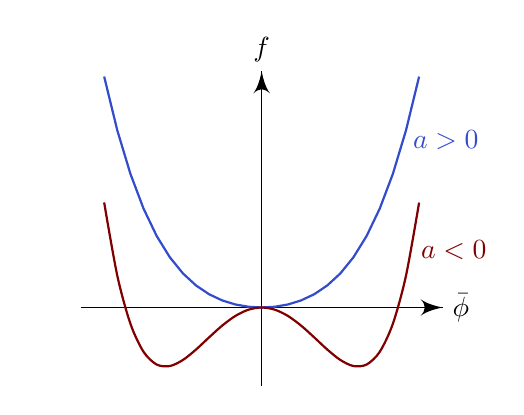
\begin{tikzpicture}
    \draw [->] (-2.3, 0) -- (2.3, 0) node [right] {$\bar{\phi}$};
    \draw [->] (0, -1) -- (0, 3) node [above] {$f$};
    \draw [domain=-2:2, mblue, thick] plot (\x, {(\x)^2/3 + (\x)^4/10});
    \draw [domain=-2:2, mred, thick] plot [smooth] (\x, {-(\x)^2 + (\x)^4/3});

    \node [right, mblue] at (1.8, 2.13) {$a > 0$};
    \node [right, mred] at (1.9, 0.734) {$a < 0$};
    \node [left, white] at (-1.8, 2.13) {$a > 0$};
    \node [left, white] at (-1.9, 0.734) {$a < 0$};
  \end{tikzpicture}
\end{center}
It is the $a < 0$ case that is interesting. The two minima lie at $\phi_{1, 2} = \pm \phi_B$, where
\[
  \phi_B = \sqrt{\frac{-a}{b}}.
\]
Now suppose $\bar{\phi}$ lies between $\pm \phi_B$. Then it might be advantageous to have some parts of the fluid being at $-\phi_B$ and the others at $\phi_B$, and join them smoothly in between to control the gradient term. Mathematically, this is captured by the concavity of the function $f$ in the region $[-\phi_B, \phi_B]$, i.e.\ if there are $V_1$ many fluids with $\phi = \phi_1$, and $V_2$ many fluids with $\phi = \phi_2$, so that
\begin{align*}
  V_1 \phi_1 + V_2 \phi_2 &= V \bar{\phi},\\
  V_1 + V_2 &= V,
\end{align*}
then we have
\[
  V_1 f(\phi_1) + V_2 f(\phi_2) < (V_1 + V_2) f(\bar{\phi}).
\]
This phase separated state has a lower energy than the single phase version, at least if the gradient term is well-controlled.

In general the mean-field phase diagram looks like
\begin{center}
  \begin{tikzpicture}
    \draw (-2, 3) node [above] {$a$} -- (-2, 0) node [below] {$-1$} -- (2, 0) node [below] {$1$} node [right] {$\bar \phi$} -- (2, 3);
    \node [left] at (-2, 2.5) {$a(T) = 0$};

    \draw [domain=2.5:0.2, samples=40] plot [smooth] ({sqrt (2.5 - \x)}, \x);
    \draw [domain=2.5:0.2, samples=40] plot [smooth] ({-sqrt (2.5 - \x)}, \x);

    \draw [dashed, domain=0.2:2.5] plot [smooth] ({sqrt ((2.5 - \x)/3)}, \x);
    \draw [dashed, domain=0.2:2.5] plot [smooth] ({-sqrt ((2.5 - \x)/3)}, \x);
    \draw (-2.05, 2.5) -- (-1.95, 2.5);
  \end{tikzpicture}
\end{center}
Within the solid lines, we have phase separation, where the ground state of the system for the given $a$ and $\bar{\phi}$ is given by the state described above. The inner curve denotes \term{spinodal instability}, where we in fact have local instability, as opposed to global instability. This is given by the condition $f''(\bar{\phi}) < 0$, which we solve to be
\[
  \phi_S = \sqrt{\frac{-a}{3b}}.
\]

What happens if our fluid is no longer symmetric? In this case, we should add odd terms as well. As we previously discussed, a linear term has no effect. How about a cubic term $\int \frac{c}{3} \phi(\mathbf{r})^3 \;\d \mathbf{r}$ to our $\beta F$? It turns out we can remove the $\phi(\mathbf{r})$ term by a linear shift of $\phi$ and $a$, which is a simple algebraic maneuver. So we have a shift of axes on the phase diagram, and nothing interesting really happens.

\subsection{Nematic liquid crystals}
There are two basic ways of organizing rod-like molecules --- \term{isotropic} and \term{nematic}. In the first case, the rods are pointed in random directions, whereas in the nematic case, the rods all point in the same direction, i.e.\ there is a long range orientation order. However, there is no long-range positional order.

In the case of hard rods, we transition from isotropic to nematic when the density $\rho$ is increased.

The first and perhaps subtle point is that we have to pick an order parameter. Nematic molecules have a preferred \emph{axis}, but not a \emph{sense}, i.e.\ we can rotate our rod by $180^\circ$ and it still looks the same. Thus the orientation is represented by a ``headless vector'' $\nu$. Instead, it takes values in real projective space.

Given an arbitrary vector $A$, and $\mathbf{n}$ the direction of our rod, we can write down $(A \cdot \mathbf{n}) \mathbf{n}$ is the component of $\mathbf{A}$ along $\mathbf{n}$. While $A_i n_i n_j$ is a vector, $n_i n_j$ is a second-rank tensor, whose trace is $1$ (as $n$ is a unit vector). Crucially, if we flip the sign of all components of $n$, this does not change. If we have isotropic rods, then
\[
  \bra n_i n_j \ket = \frac{\delta_{ij}}{d},
\]
where $d$ is the number of dimensions. This allows us to introduce an order parameter
\[
  Q_{ij} (\mathbf{r}) = \bra n_i n_j\ket_{local} - \frac{1}{d} \delta_{ij}.
\]
Again, we need to pick a scale to do the coarse-graining. This is a traceless symmetric second-rank tensor, and vanishes in the isotropic phase, and non-zero in the nematic phase.

An interesting thing about this is that it is not conserved, i.e.\ $\int Q_{ij}(\mathbf{r})\;\d \mathbf{r}$ is not constant in time. This will have consequences for equilibrium statistical mechanics, but also the dynamics. So this is quite different from our previous binary fluid. We can follow the same procedure as we previously did, but it is going to be more complicated.

We have a free energy function. We start with the local part $f(Q)$, which is a scalar built on $Q$ via a Taylor series. So we need to find scalar invariants of $Q$.
\begin{enumerate}
  \item There is only one linear one, namely $Q_{ii} = \Tr(Q)$, but this vanishes.
  \item We can construct a quadratic term $Q_{ij} Q_{ji} = \Tr(Q^2)$, and this is in general non-zero.
  \item There is a cubic term $Q_{ij} Q_{jk} Q_{ki} = \Tr(Q^3)$, and is also in general non-zero.
  \item There are two possible quartic terms, namely $\Tr(Q^2)^2$ and $\Tr(Q^4)$.
\end{enumerate}
So we can write
\[
  f(Q) = a\Tr(Q^2) + c \Tr(Q^3) + b_1 \Tr(Q^2)^2 + b_2 \Tr(Q^4).
\]
This is the local part of the free energy up to fourth order in $Q$. We can go on, and in certain conditions we have to go on, but if these coefficients $b_i$ are sufficiently positive in some sense, we don't have to.

What can we say about the cubic term? Under what conditions do we expect $c$ to vanish? To understand this better, we fix $d = 3$, and consider the configuration
\[
  Q_{ij} =
  \begin{pmatrix}
    -\lambda/2 & 0 & 0\\
    0 & -\lambda/2 & 0\\
    0 & 0 & \lambda
  \end{pmatrix},\quad \lambda > 0.
\]
This arises if, for example, uniformly over the material, the rods are all likely to point in the $z$-direction. If $\lambda < 0$ instead, then the rods are all \emph{un}likely to point in the $z$-direction. There is absolutely no reason for these two states to have similar free energy, and the difference between the two is only captured in odd terms.

In the first example, we have
\begin{align*}
  f(Q) &= a \left(\frac{3}{2} \lambda^2\right) + c \left(\frac{3}{4} \lambda^3\right) + b_1\left(\frac{9}{4} \lambda^4\right) + b_2 \left(\frac{9}{8} \lambda^4\right)\\
  &= \bar{a} \lambda^2 + \bar{c} \lambda^3 + \bar{b}\lambda^4.
\end{align*}
This, we can think of this in a way similar to the binary fluid, where $\lambda$ is are sole order parameter. As a function of $\lambda$, where we vary $\bar{a}$ and fix $\bar{b}$ and $\bar{c} < 0$, we have
\begin{center}
  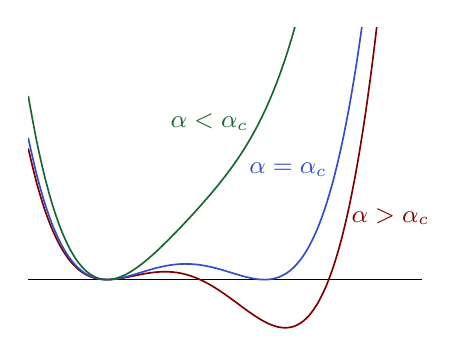
\begin{tikzpicture}[yscale=4]
    \draw (-1, 0) -- (4, 0);
    \clip (-1, -0.16) rectangle (4.3, 0.8);
    \draw [domain=-1:4, samples=50, mred, semithick] plot [smooth] (\x, {(\x)^2/6 - (\x)^3/5 + (\x)^4 / 20});
    \draw [domain=-1:4, samples=50, mblue, semithick] plot [smooth] (\x, {(\x)^2/5 - (\x)^3/5 + (\x)^4 / 20});
    \draw [domain=-1:4, samples=50, mgreen, semithick] plot [smooth] (\x, {(\x)^2/3 - (\x)^3/5 + (\x)^4 / 20});

    \node [mgreen] at (1.3, 0.5) {\small$\alpha < \alpha_c$};
    \node [mblue] at (2.3, 0.35) {\small$\alpha = \alpha_c$};
    \node [mred] at (3.6, 0.2) {\small$\alpha > \alpha_c$};
  \end{tikzpicture}
\end{center}
Here the cubic term gives a discontinuous transition. This is a first-order transition. If we had $\bar{c} > 0$ instead, then the minima are on the other side.

In general, cubic terms lead to discontinuous transitions.

We now move on to the gradient terms. We can have something of the form
\[
  F[Q] = \int \big(f(Q) + f_{\ell i}(\nabla_i Q_{kj})\big)\;\d \mathbf{r}.
\]
We do this to order $\nabla^{(2)}$ and $Q^{(2)}$. The only possible combinations are
\begin{align*}
  \kappa_1 \nabla_i \nabla_i Q_{j\ell} Q_{j\ell} &= \kappa_1 \nabla^2 \Tr(Q^2) \\
  \kappa_2 (\nabla_i Q_{im}) (\nabla_j Q_{jm}) &= \kappa_2(\nabla \cdot Q)^2\\
  \kappa_3 (\nabla_i Q_{jm}) (\nabla_j Q_{im}) &= \text{yuck}.
\end{align*}
Three linear combinations describe the following three things:
\begin{center}
  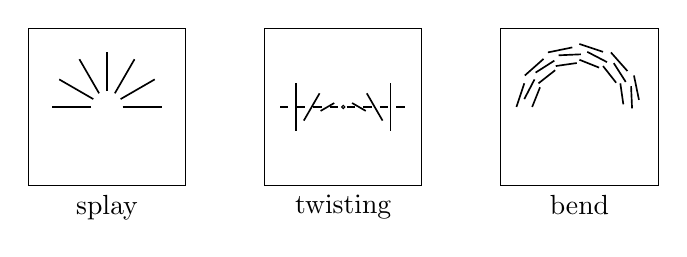
\begin{tikzpicture}
    \begin{scope}
      \draw (-1, -1) rectangle (1, 1);
      \node [below] at (0, -1) {splay};

      \draw [semithick] (0, 0.2) -- +(0, 0.5);
      \draw [semithick, rotate=30] (0, 0.2) -- +(0, 0.5);
      \draw [semithick, rotate=60] (0, 0.2) -- +(0, 0.5);
      \draw [semithick, rotate=90] (0, 0.2) -- +(0, 0.5);
      \draw [semithick, rotate=-30] (0, 0.2) -- +(0, 0.5);
      \draw [semithick, rotate=-60] (0, 0.2) -- +(0, 0.5);
      \draw [semithick, rotate=-90] (0, 0.2) -- +(0, 0.5);
    \end{scope}
    \begin{scope}[shift={(3, 0)}]
      \draw (-1, -1) rectangle (1, 1);
      \node [below] at (0, -1) {twisting};

      \draw [semithick] (-0.6, -0.3) -- +(0, 0.6);
      \draw [semithick] (0.6, -0.3) -- +(0, 0.6);

      \draw [semithick, rotate around={-30:(-0.4,0)}] (-0.4, -0.2) -- +(0, 0.4);
      \draw [semithick, rotate around={-60:(-0.2,0)}] (-0.2, -0.1) -- +(0, 0.2);

      \draw [semithick, rotate around={30:(0.4,0)}] (0.4, -0.2) -- +(0, 0.4);
      \draw [semithick, rotate around={60:(0.2,0)}] (0.2, -0.1) -- +(0, 0.2);

      \draw (0, 0) circle [radius=0.02];

      \draw [dashed, thin] (-0.8, 0) -- (0.8, 0);
    \end{scope}
    \begin{scope}[shift={(6, 0)}]
      \draw (-1, -1) rectangle (1, 1);
      \node [below] at (0, -1) {bend};

      \draw [semithick] (-0.8, 0) -- (-0.7, 0.3);
      \draw [semithick, rotate=-30] (-0.8, 0) -- (-0.7, 0.3);
      \draw [semithick, rotate=-60] (-0.8, 0) -- (-0.7, 0.3);
      \draw [semithick, rotate=-90] (-0.8, 0) -- (-0.7, 0.3);
      \draw [semithick, rotate=-120] (-0.8, 0) -- (-0.7, 0.3);
      \draw [semithick, rotate=-150] (-0.8, 0) -- (-0.7, 0.3);

      \draw [semithick] (-0.7, 0.1) -- (-0.57, 0.35);
      \draw [semithick, rotate=-30] (-0.7, 0.1) -- (-0.57, 0.35);
      \draw [semithick, rotate=-60] (-0.7, 0.1) -- (-0.57, 0.35);
      \draw [semithick, rotate=-90] (-0.7, 0.1) -- (-0.57, 0.35);
      \draw [semithick, rotate=-120] (-0.7, 0.1) -- (-0.57, 0.35);
      \draw [semithick, rotate=-150] (-0.7, 0.1) -- (-0.57, 0.35);

      \draw [semithick] (-0.6, 0) -- (-0.5, 0.25);
      \draw [semithick, rotate=-30] (-0.6, 0) -- (-0.5, 0.25);
      \draw [semithick, rotate=-60] (-0.6, 0) -- (-0.5, 0.25);
      \draw [semithick, rotate=-90] (-0.6, 0) -- (-0.5, 0.25);
      \draw [semithick, rotate=-120] (-0.6, 0) -- (-0.5, 0.25);
      \draw [semithick, rotate=-150] (-0.6, 0) -- (-0.5, 0.25);
    \end{scope}
  \end{tikzpicture}
\end{center}
Individually, we cannot see which $\kappa_i$ correspond to which modes, but they are given by some linear combinations.

The usual (simplest) choice is to set $\kappa_1 = \kappa_3 = 0$. If we make that choice, we find that there is a similar elastic cost to each of these deformations.

\section{Functional Integrals}
\subsection{Functional derivatives}
Before we do functional integrals, we review a bit of functional differentiation. Consider a scalar field $\varphi(\mathbf{r})$, and consider a functional
\[
  A[\phi] = \int L(\phi, \nabla \phi)\;\d \mathbf{r}.
\]
Consider a small change $\phi \mapsto \phi + \delta \phi(\mathbf{r})$, and we require $\delta \phi = 0$ on the boundary. Then
\begin{align*}
  A[\phi + \delta \phi] &= \int \left(L(\phi, \nabla \phi) + \delta \phi \frac{\partial L}{\partial \phi} + \nabla d \phi \cdot \frac{\partial L}{\partial \phi}\right)\;\d \mathbf{r}\\
  &= A[\phi] + \int \delta \phi \left(\frac{\partial L}{\partial \phi} + \nabla \cdot \frac{\partial L}{\partial \nabla \phi}\right)\;\d \mathbf{r},
\end{align*}
where we integrated by parts using the boundary condition. We then define\index{functional derivative}\index{$\frac{\delta A}{\delta \phi(\mathbf{r})}$}
\[
  \frac{\delta A}{\delta \phi(\mathbf{r})} = \frac{\partial L}{\partial \phi(\mathbf{r})} - \nabla \cdot \frac{\partial L}{\partial \nabla \phi}.
\]
\begin{eg}
  In classical mechanics, we replace $\mathbf{r}$ by the single variable $t$, and $\phi$ by position $x$. We then have
  \[
    A = \int L(x, \dot{x})\;\d t.
  \]
  Then we have
  \[
    \frac{\delta A}{\delta x(t)} = \frac{\partial L}{\partial x} - \frac{\d}{\d t} \left(\frac{\partial L}{\partial \dot{x}}\right),
  \]
  and in classical mechanics, we set this to zero.
\end{eg}

The example more relevant to us is perhaps Landau--Ginzburg theory:
\begin{eg}
  Consider a coarse-grained free energy
  \[
    F[\phi] = \int \left(\frac{a}{2} \phi^2 + \frac{b}{4} \phi^4 + \frac{\kappa}{2} (\nabla \phi)^2 \right)\;\d \mathbf{r}.
  \]
  Then
  \[
    \frac{\delta F}{\delta \phi(\mathbf{r})} = a \phi + b \phi^3 - \kappa \nabla^2 \phi.
  \]
  In mean field theory, we set this to zero, since by definition, we are choosing a single $\phi(\mathbf{r})$ that minimizes $F$. In the example sheet, we solve this to get
  \[
    \phi(x) = \phi_B \tanh \left(\frac{x - x_0}{\xi_0}\right).
  \]
\end{eg}

For a general $F[\psi]$, we can think of the functional derivative $\frac{\delta F}{\delta \psi(\mathbf{r})}$ as a ``generalized force'', and it tells the system which way to move in order to reduce the free energy. Recall that
\[
  \d F = - S \;\d T - p \;\d V + \mu \;\d N + \mathbf{h} \cdot \d \mathbf{M} + \cdots.
\]
We can then think of
\[
  \delta F = \int \frac{\delta F}{\delta \psi(\mathbf{r})} \delta \psi(\mathbf{r})\;\d r.
\]
as an additional term, and we can think of $\frac{\delta F}{\delta \psi(\mathbf{r})}$ as the intensive variable, while $\delta \psi(\mathbf{r})$ is the extensive variable. If $\psi$ is the particle density, for example, then we can think of these as the $\mu$ and $N$ respectively. If it is the magnetization, then these would be like $\mathbf{h}$ and $\mathbf{M}$.

Note that for $\psi$ a conserved scalar density $(\rho, \phi)$, the quantity
\[
  \mu(\mathbf{r}) = \frac{\delta F}{\delta \phi(\mathbf{r})}
\]
is called the \term{chemical potential}.

On the other hand, if $\psi$ is not conserved, e.g.\ the $Q$ we had before, then
\[
  H_{ij} = \frac{\delta F}{\delta Q_{ij}}
\]
is called the \emph{molecular field}.

In the case where $\phi$ is conserved, we have the conservation law
\[
  \dot{\phi} = - \nabla \cdot J.
\]
This $J$ is then given by an equation of the form
\[
  J \propto -D \nabla \mu,
\]
where $D$ is the diffusivity.

The non-conserved case is simpler. We have
\[
  \dot{Q} = - \Gamma H.
\]
This is local relaxation.

Let us go back to the scalar field $\phi(\mathbf{r})$. Consider a small displacement
\[
  \mathbf{r} \mapsto \mathbf{r} + \mathbf{u}(\mathbf{r}).
\]
We take this to be incompressible, so that $\nabla \cdot \mathbf{u} = 0$. Then
\[
  \phi \mapsto \phi' = \phi'(\mathbf{r}) = \phi(\mathbf{r} - \mathbf{u}).
\]
Then
\[
  \delta \phi(\mathbf{r}) = \phi'(\mathbf{r}) - \phi(\mathbf{r}) = - \mathbf{u} \cdot \nabla \phi(\mathbf{r}) + O(u^2).
\]
Then
\begin{align*}
  \delta F &= \int \delta \phi \frac{\delta F}{\delta \phi}\;\d \mathbf{r} \\
  &= -\int \mu \mathbf{u} \cdot \nabla \phi \;\d \mathbf{r}\\
  &= \int \phi \nabla \cdot (\mu \mathbf{u})\;\d \mathbf{r}\\
  &= \int (\phi \nabla \mu)\cdot \mathbf{u}\;\d \mathbf{r}\\
  &= \int (\phi \nabla_j \mu)u_j\;\d \mathbf{r}.
\end{align*}
using incompressibility.

We can think of the free energy change as the work done by stress,
\[
  \delta F = \int \sigma_{ij}(\mathbf{r}) \varepsilon_{ij}(\mathbf{r})\;\d \mathbf{r},
\]
where $\varepsilon_{ij} = \nabla_i u_j$ is the strain tensor, and $\sigma_{ij}$ is the stress tensor. So we can write this as
\[
  \delta F = \int \sigma_{ij} \nabla_i u_j\;\d \mathbf{r} = - \int (\nabla_i \sigma_{ij}) u_j\;\d \mathbf{r}.
\]
So we can identify
\[
  \nabla_i \sigma_{ij} = -\phi \nabla_j \mu.
\]
So $\mu$ also contains the ``mechanical information''.

\subsection{Functional integrals}
Given a coarse-grained $\psi$, we have can define the total partition function
\[
  e^{-\beta F_{TOT}} = Z_{TOT} = \int e^{-\beta F[\psi]} \;\D [\psi],
\]
where $\D [\psi]$ is the ``sum over all field configurations''. In mean field theory, we approximate this $F_{TOT}$ by replacing the functional integral by the value of the integrand at its maximum, i.e.\ taking the minimum value of $F[\psi]$. What we are going to do now is to evaluate the functional integral ``honestly'', and this amounts to taking into account fluctuations around the minimum (since those far away from the minimum should contribute really little).

To make sense of the integral, we use the fact that the space of all $\psi$ has a countable basis, given by the Fourier modes. We define $\psi_\mathbf{q}$ by setting
\[
  \psi_\mathbf{q} = \frac{1}{\sqrt{V}} \int \psi(\mathbf{r}) e^{-i\mathbf{q}\cdot \mathbf{r}}\;\d \mathbf{r},
\]
where $V = L^q$ is our region with periodic boundary conditions. Note that in such a periodified world, $\mathbf{q}$ can only take on a set of discrete values. The protocol is to keep $V < \infty$ until we are done with all calculations, and then take the thermodynamic limit $V \to \infty$ if we want. In this limit, the sum over $\mathbf{q}$ becomes an integral, and it is harder to make sense of $\D[\psi]$.

The normalization of $\psi_\mathbf{q}$ is chosen so that
\[
  \int |\psi|^2 \;\d \mathbf{r} = \sum_{\mathbf{q} } |\psi_\mathbf{q}|^2.
\]
This is known as \term{Parseval's theorem}. We can then define
\[
  \D [\psi] = \prod_{\mathbf{q}} \;\d \psi_\mathbf{q}.
\]
An infinite product is still bad, but usually molecular physics or the nature of coarse graining imposes a maximum $q_{max}$, and we take the product up to there. In most of our calculations, we need such a $q_{max}$ to make sense of our integrals, and that will be left implicit. Most of the time, the results will be independent of $q_{max}$ (for example, it may give rise to a constant shift to $F$ that is independent of all the variables of interest).

Another point to note is that if $\psi$ is a real variable, then not all $\psi_\mathbf{q}$ are independent. They are related by
\[
  \psi_\mathbf{q} = \psi_{-\mathbf{q}}^*.
\]
Thus, we should only multiply over half of the possible $\mathbf{q}$'s, and we usually denote this by something like $\prod^+_{\mathbf{q}}$.

In practice, there is only one integral like this that can be done, namely when $\beta F$ is a quadratic form. Consider a free energy of the form
\[
  \beta F = \frac{1}{2} \int \phi(\mathbf{r}) G(\mathbf{r} - \mathbf{r}') \phi(\mathbf{r}')\;\d \mathbf{r}\;\d \mathbf{r}' - \int h(\mathbf{r}) \phi(\mathbf{r})\;\d \mathbf{r}.
\]
We can think of the gradient terms we previously had as localizations of first-order approximations to the non-local interactions. Taking the Fourier transform, we get
\[
  \beta F[\psi_\mathbf{q}] = \frac{1}{2} \sum_q G(\mathbf{q}) \phi_\mathbf{q} \phi_{-\mathbf{q}} - \sum_\mathbf{q} h_\mathbf{q} \phi_\mathbf{q}.
\]
\begin{eg}
  We take Landau--Ginzburg theory and consider terms of the form
  \[
    \beta F[\phi] = \int \left\{\xi \phi^2 - h \phi + \frac{\kappa}{2} (\nabla \phi)^2 + \frac{\gamma}{2} (\nabla^2 \phi)^2\right\}\;\d \mathbf{r}
  \]
  and then we set $b = 0$ since this is the scenario we know how to deal with. We will later see how we can put it back. The $\gamma$ term is necessary because we will be interested in the case where $\kappa$ is negative.

  We can now take the Fourier transform to get
  \begin{align*}
    \beta F \{\phi_\mathbf{q}\} &= \frac{1}{2} \sum_\mathbf{q} (a + \kappa q^2 + \gamma q^4) \phi_\mathbf{q} \phi_{-\mathbf{q}} - \sum_\mathbf{q} h_\mathbf{q} \phi_\mathbf{q}.\\
    &= \sum_\mathbf{q}\splus (a + \kappa q^2 + \gamma q^4) \phi_\mathbf{q} \phi_{-\mathbf{q}} - \sum_\mathbf{q} h_\mathbf{q} \phi_\mathbf{q}.
  \end{align*}
  So our $G(\mathbf{q})$ is given by
  \[
    G(\mathbf{q}) = a + k q^2 + \gamma q^4.
  \]
\end{eg}
To actually perform the functional integral, first note that if $h \not= 0$, then we can complete the square so that the $h$ term goes away. So we may assume $h = 0$. We then have
\begin{align*}
  Z_{TOT} &= \int \left[ \prod_{\mathbf{q}}\splus \;\d \phi_\mathbf{q}\right] e^{-\beta F\{\phi_\mathbf{q}\}}\\
  &= \prod_\mathbf{q}\splus \int \d \phi_\mathbf{q} e^{-|\phi_\mathbf{q}|^2 G(q)}
\end{align*}
Each individual integral can be evaluated as
\[
  \int \d \phi_\mathbf{q}\;e^{-|\phi_\mathbf{q}|^2 G(q)} = \int \rho \;\d \rho \;\d \theta\; e^{-G(q) \rho^2} = \frac{\pi}{G(q)},
\]
where $\phi_\mathbf{q} = \rho e^{i\theta}$. So we find that
\[
  Z_{TOT} = \prod_\mathbf{q}\splus \frac{\pi}{G(q)},
\]
and so
\[
  \beta F_T = -\log Z_T = \sum_\mathbf{q}\splus \log \frac{G(q)}{\pi}.
\]
We now take large $V$ limit, and replace the sum of the integral. Then we get
\[
  \beta F_T = \frac{1}{2} \frac{V}{(2\pi)^d} \int^{q_{max}} \d \mathbf{q}\;\log \frac{G(q)}{\pi}.
\]
There are many quantities we can compute from the free energy.
\begin{eg}
  The \term{structure factor} is defined to be
  \[
    S(\mathbf{k}) = \bra \phi_\mathbf{k} \phi_{-\mathbf{k}}\ket = \frac{1}{Z_T} \int \phi_\mathbf{k} \phi_{-\mathbf{k}} e^{-\sum_\mathbf{q}^+ \phi_\mathbf{q} \phi_{-\mathbf{q}} G(q)} \prod_q\splus \;\d \phi_\mathbf{q}.
  \]
  We see that this is equal to
  \[
    \frac{1}{Z_T} \frac{\partial Z_T}{\partial G(\mathbf{k})} = - \frac{\partial \log Z_T}{\partial G(\mathbf{k})} = \frac{1}{G(k)}.
  \]
  Note that we could also have done this explicitly using the product expansion.

  This $S(k)$ is measured in scattering experiments. In our previous example, for small $k$ and $\kappa > 0$, we have
  \[
    S(q) = \frac{1}{a + \kappa k^2 + \gamma k^4} \approx \frac{a^{-1}}{1 + k^2 \xi^2},
  \]
  where $\xi$ is the \term{correlation length}, given by
  \[
    \xi = \sqrt{\frac{\kappa}{a}}.
  \]
  We can return to real space by
  \begin{align*}
    \bra \phi^2(\mathbf{r})\ket &= \frac{1}{V} \left\bra \int |\phi(\mathbf{r})|^2 \;\d \mathbf{r}\right\ket \\
    &= \frac{1}{V} \sum_q \bra \phi_\mathbf{q}|^2\ket\\
    &= \frac{1}{(2\pi)^d} \int^{q_{max}} \frac{\d \mathbf{q}}{a + \kappa q^2 + \gamma q^4}.
  \end{align*}
\end{eg}

\subsection{The variational method}
What can we do when our free energy is not quadratic? What we previously did was to do mean field theory, but we know this fails near the critical point. In Statistical Field Theory, we used renormalization group methods. Here we go for something in between, namely the variational method. In condensed matter physics, this is known as \term{Hartree theory}, and in QFT it is known as ``\term{1-loop self consistency}''. This theory handles large Gaussian fluctuations well, and we shall use it to study smectic liquid crystals.

For simplicity, we set $\beta = 0$. Then we can write
\[
  e^{-F_{TOT}} = \int e^{-F[\phi]}\;\D [\phi].
\]
We now make a notation change, where we write $F_{TOT}$ as $F$, and we now write $F[\phi]$ as $H[\phi]$ instead, called \term{the effective Hamiltonian}. In this notation, we write
\[
  e^{-F} = \int e^{-H[\phi]} \;\D [\phi].
\]
In the variational method, we introduce a \term{trial Hamiltonian} $H_0[\phi]$, which is one we understand well. We can similarly define
\[
  e^{-F_0} = \int e^{-H_0[\phi]} \;\D [\phi].
\]
We can then write
\begin{align*}
  e^{-F} &= \frac{e^{-F_0}}{\int e^{-H_0}\;\D [\phi]} \int e^{-H_0} e^{-(H - H_0)}\;\D [\phi] \\
  &= e^{-F_0} \bra e^{-(H - H_0)} \ket_0,
\end{align*}
where we are taking the average over the trial distribution. Taking the logarithm, we end up with
\[
  F = F_0 - \log \bra e^{-(H - H_0)}\ket_0.
\]
So far, everything is exact, and this manipulation doesn't help much. The useful approximation comes from observing that the function $\log$ is concave. In other words,
\[
  \log (\alpha A + (1 - \alpha) B) \geq \alpha \log A + (1 - \alpha) \log B.
\]
Hence by Jensen's inequality, we have
\[
  \log \bra Y \ket_0 \geq \bra \log Y \ket_0.
\]
Applying this to our situation gives us an inequality
\[
  F \leq F_0 - \bra H_0 - H\ket_0 = F_0 - \bra H_0\ket_0 + \bra H\ket_0 = S_0 + \bra H\ket_0.
\]
This is the \term{Feynman--Bogoliubov inequality}.

To use this, we have to choose the trial distribution $H_0$ simple enough to actually do calculations (i.e.\ Gaussian), but include variational parameters in $H_0$. We then minimize the quantity $F_0 - \bra H_0\ket + \bra H\ket_0$ over our variational parameters, and this gives us an upper bound on $F$. We then take this to be our best estimate of $F$.

\subsection{Smectic liquid crystals}
We use this to talk about the isotropic to smectic transition in liquid crystals. The molecules involved often have two distinct segments. For example, we may have soap molecules that look like this:
\begin{center}
  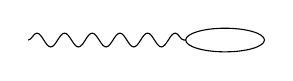
\begin{tikzpicture}
    \draw (3, 0) ellipse (0.5 and 0.15);
    \draw [decorate, decoration=snake] (0.5, 0) -- (2.5, 0);
  \end{tikzpicture}
\end{center}
The key property of soap molecules is that the tail hates water while the head likes water. So we expect these molecules to group together like
\begin{center}
  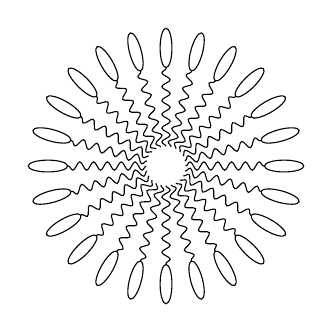
\begin{tikzpicture}[scale=0.5]
    \foreach \r in {0,15,...,345} {
      \begin{scope}[rotate=\r]
        \draw (3, 0) ellipse (0.5 and 0.15);
        \draw [decorate, decoration={snake, amplitude=1.5, segment length=5}] (0.5, 0) -- (2.5, 0);
      \end{scope}
  }
  \end{tikzpicture}
\end{center}
In general, we can imagine our molecules look like
\begin{center}
  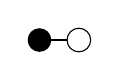
\begin{tikzpicture}[rotate=90, scale=0.5]
    \fill circle [radius=0.3];
    \draw (0, -1) circle [radius=0.3];
    \draw (0, -0.3) -- (0, -0.7);
  \end{tikzpicture}
\end{center}
and like attracts like. As in the binary fluid, we shall assume the two heads are symmetric, so $U_{AA} = U_{BB} \not= U_{AB}$. If we simply want the different parts to stay away from each other, then we can have a configuration that looks like
\begin{center}
  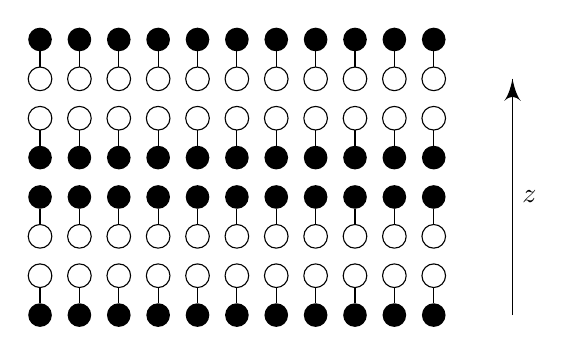
\begin{tikzpicture}[scale=0.5]
    \foreach \x in {0,...,10} {
      \foreach \y in {0,4} {
        \begin{scope}[shift={(\x, \y)}]
          \fill circle [radius=0.3];
          \draw (0, -1) circle [radius=0.3];
          \draw (0, -2) circle [radius=0.3];
          \fill (0, -3) circle [radius=0.3];
          \draw (0, -0.3) -- (0, -0.7);
          \draw (0, -2.3) -- (0, -2.7);
        \end{scope}
      }
   }
   \draw [->] (12, -3) -- (12, 3) node [pos=0.5, right] {$z$};
  \end{tikzpicture}
\end{center}
In general, we expect that there is such an order along the $z$ direction, as indicated, while there is no restriction on the alignments in the other directions. So the system is a lattice in the $z$ direction, and a fluid in the remaining two directions. This is known as a \term{smectic liquid crystal}, and is also known as the \term{lamellar phase}. This is an example of \term{microphase separation}.

As before, we let $\phi$ be a coarse grained relative density. The above ordered phase would then look like
\[
  \phi(\mathbf{x}) = \cos q_0 z.
\]
for some $q_0$ that comes from the molecular length. If our system is not perfectly ordered, then we may expect it to look roughly like $A \cos q_0 z$ for some $A$.

We again use Landau--Ginzburg model, which, in our old notation, has
\[
  \beta F = \int \left(\frac{a}{2} \phi^2 + \frac{b}{4} \phi^4 + \frac{\kappa}{2} (\nabla \phi)^2 + \frac{\gamma}{2} (\nabla^2 \phi)^2\right)\;\d \mathbf{r}.
\]
If we write this in Fourier space, then we get
\[
  \beta F = \frac{1}{2} \sum_{\mathbf{q}} (a + \kappa q^2 + \gamma q^4) \phi_{\mathbf{q}} \phi_{-\mathbf{q}} + \frac{b}{4V} \sum_{\mathbf{q}_1, \mathbf{q}_2, \mathbf{q}_3} \phi_{\mathbf{q}_1} \phi_{\mathbf{q}_2} \phi_{\mathbf{q}_3} \phi_{-(\mathbf{q}_1 + \mathbf{q}_2 + \mathbf{q}_3)}.
\]
Notice that the quartic term results in the rather messy sum at the end. For the iso-smectic transition, we choose $\kappa < 0, \gamma > 0$.

Again for simplicity, we first consider the case where $b = 0$. Then this is a Gaussian model with
\[
  G(q) = a + \kappa q^2 + \gamma q^4 = \tau + \alpha(q - q_0)^2,
\]
Varying $a$ gives a linear shift in $G(q)$. As we change $a$, we get multiple different curves.
\begin{center}
  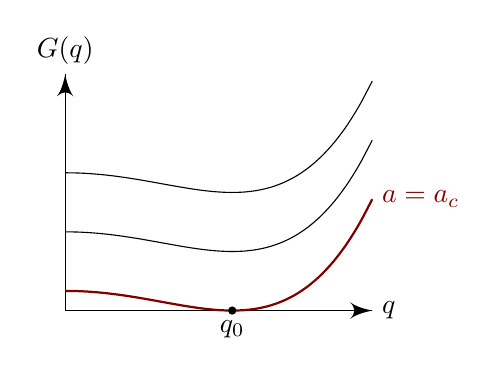
\begin{tikzpicture}[xscale=3]
    \draw [->] (0, 0) -- (1.3, 0) node [right] {$q$};
    \draw [->] (0 ,0) -- (0, 3) node [above] {$G(q)$};

    \draw [domain=0:1.3] plot [smooth] (\x, {1 - \x^2 + \x^4});
    \draw [domain=0:1.3, thick, mred] plot [smooth] (\x, {0.25 - \x^2 + \x^4});
    \draw [domain=0:1.3] plot [smooth] (\x, {1.75 - \x^2 + \x^4});
    \node [right, mred] at (1.3, 1.4161) {$a = a_c$};

    \node [circ] at (0.707, 0) {};
    \node [below] at (0.707, 0) {$q_0$};
  \end{tikzpicture}
\end{center}
Thus, as $a$ decreases, $S(q) = \bra |\phi_\mathbf{q}|^2 \ket = \frac{1}{G(q)}$ blows up at some finite
\[
  q = q_0 = \sqrt{\frac{-\kappa}{2\gamma}},\quad a_c = \frac{\kappa^2}{4 \gamma}.
\]
We should take this blowing up as saying that the $|\mathbf{q}| = q_0$ states are highly desired, and this results in an ordered phase. Note that \emph{any} $\mathbf{q}$ with $|\mathbf{q}| = q_0$ is highly desired. When the system actually settles to an ordered state, it has to \emph{pick} one such $\mathbf{q}$ and let the system align in that direction. This is \term{spontaneous symmetry breaking}.

It is convenient to complete to square, and expand $G$ about $q = q_0$ and $a = a_c$. Then we have
\[
  G(q) = \tau + \alpha(q - q_0)^2,
\]
where
\[
  \tau = a - a_c,\quad \alpha = \frac{1}{2} G''(q_0) = - 2\kappa.
\]
Then the transition we saw above happens when $\tau = 0$.

We now put back the quartic term. We first do this with mean field theory, and then later return to the variational method.
\subsubsection*{Mean Field Theory}
In mean field theory, it is easier to work in real space. We look for a single field configuration that minimizes $F$. As suggested before, we try a solution of the form
\[
  \phi = A \cos q_0 z,
\]
which is smectic along $z$. We can then evaluate the free energy (per unit volume) to be
\[
  \frac{\beta F}{V} = \beta \overline{F[\phi]} = \frac{a}{2} \overline{\phi^2} + \frac{\kappa}{2} \overline{(\nabla \phi)^2} + \frac{\gamma}{2} \overline{(\nabla^2 \phi)^2} + \frac{b}{4} \overline{\phi^4}
\]
where the bar means we average over one period of the periodic structure. It is an exercise to directly compute
\[
  \overline{\phi^2} = \frac{1}{2} A^2,\quad \overline{(\nabla \phi)^2} = \frac{1}{2} A^2 q_0^2,\quad \overline{(\nabla^2 \phi)^2} =\frac{1}{2} A^2 q_0^4,\quad \overline{\phi^4} = \frac{3}{8} A^4.
\]
This gives
\[
  \frac{\beta F}{V} = \frac{1}{4} \left[aA^2 + \kappa A^2 q_0^2 + \gamma A^2 q_0^4 + \frac{3b}{8} A^4\right] = \frac{1}{4} \left[ A^2 \underbrace{(a - a_c)}_\tau + \frac{3b}{8} A^4\right].
\]
Note that $q_0$ is fixed by the system as we originally had, while $A$ is the amplitude of the fluctuation which we get to choose. Plotting this, we get a familiar graph
\begin{center}
  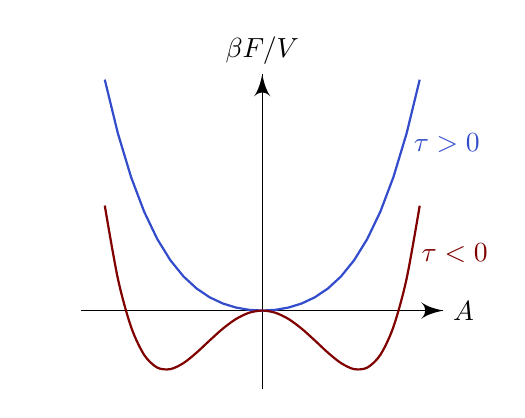
\begin{tikzpicture}
    \draw [->] (-2.3, 0) -- (2.3, 0) node [right] {$A$};
    \draw [->] (0, -1) -- (0, 3) node [above] {$\beta F/V$};
    \draw [domain=-2:2, mblue, thick] plot (\x, {(\x)^2/3 + (\x)^4/10});
    \draw [domain=-2:2, mred, thick] plot [smooth] (\x, {-(\x)^2 + (\x)^4/3});

    \node [right, mblue] at (1.8, 2.13) {$\tau > 0$};
    \node [right, mred] at (1.9, 0.734) {$\tau < 0$};
    \node [left, white] at (-1.8, 2.13) {$\tau > 0$};
    \node [left, white] at (-1.9, 0.734) {$\tau < 0$};
  \end{tikzpicture}
\end{center}
If $\tau > 0$, then the optimum solution is given by $A = 0$. Otherwise, we should pick $A \not= 0$. Observe that as we slowly reduce $\tau$ across $0$, the minimum varies \emph{continuously} with $\tau$:
\begin{center}
  \begin{tikzpicture}
    \draw [->] (0, 0) -- (4, 0) node [right] {$a$};
    \draw [->] (0, 0) -- (0, 3) node [above] {$|A|$};

    \draw [mblue, thick] (3.9, 0) -- (2, 0);
    \draw [domain=0:2, mblue, thick, samples=30] plot [smooth] (\x, {sqrt(2 - \x)});

    \node [below] at (2, 0) {$a_c$};
  \end{tikzpicture}
\end{center}
\subsubsection*{Variational method}
We now consider the variational theory. In the notation we were using previously, we have
\[
  H = \sum_\mathbf{q} \splus \phi_\mathbf{q} \phi_{-\mathbf{q}} G(q) + \frac{b}{4V} \sum_\mathbf{q} \phi_{\mathbf{q}_1} \phi_{\mathbf{q}_2} \phi_{\mathbf{q}_3} \phi_{-(\mathbf{q}_1 + \mathbf{q}_2 + \mathbf{q}_3)}.
\]
Our trial $H_0$ is
\[
  H_0 = \sum_\mathbf{q} \phi_\mathbf{q} \phi_{-\mathbf{q}} J(q).
\]
Since this is a Gaussian model, we know that
\[
  F_0 = \sum_{\mathbf{q}} \splus \log \frac{J(q)}{\pi}.
\]
To use our inequality, we need to evaluate our other two bits. We have
\[
  \bra H_0\ket_0 = \sum_{\mathbf{q}}\splus \bra \phi_\mathbf{q} \phi_{-\mathbf{q}}\ket_0 J(q).
\]
We already calculated
\[
  \bra \phi_{\mathbf{q}} \phi_{-\mathbf{q}} \ket_0 = \frac{1}{J(q)}.
\]
Thus, we have
\[
  \bra H_0 \ket_0 = \sum_{\mathbf{q}} \splus 1.
\]
Here it is clear that we must impose a cutoff on $\mathbf{q}$. We can think of this $1$ as the equipartition theorem.

We can also compute
\[
  \bra H\ket_0 = \sum_\mathbf{q} \splus \frac{1}{J(q)} G(q) + \frac{b}{4V} \underbrace{\sum_{\mathbf{q}_1, \mathbf{q}_2, \mathbf{q}_3}\bra \phi_{\mathbf{q}_1} \phi_{\mathbf{q}_2} \phi_{\mathbf{q}_3} \phi_{-(\mathbf{q}_1 \mathbf{q}_2 \mathbf{q}_3)}\ket_0}.
\]
In the Gaussian model, each $\phi_\mathbf{q}$ is a zero mean Gaussian random variables, which have certain nice properties. This is known as \term{Wick's theorem}, which tells us
\[
  \bra abcd \ket_0 = \bra ab\ket_0 \bra cd\ket_0 + \bra ac\ket_0 \bra bd\ket_0 + \bra ad\ket_0 \bra bc\ket_0.
\]
We also have
\[
  \bra \phi_{\mathbf{q}_1} \phi_{\mathbf{q}_0}\ket = \bra |\phi_\mathbf{q}|^2 \ket_0 \delta_{\mathbf{q}_1, - \mathbf{q}_2}.
\]
This gives the result
\[
  U = 3 \left[\sum_\mathbf{q} \bra |\phi_\mathbf{q}|^2\ket_0\right]^2 = 12 \left[\sum_\mathbf{q} \splus \frac{1}{J(q)}\right]^2.
\]
Thus, we have
\[
  \bra H_0\ket_0 = \sum_{\mathbf{q}} \splus \frac{G(q)}{J(q)} + \frac{3b}{V} \left(\sum_\mathbf{q} \splus \frac{1}{J(q)}\right)^2.
\]
We can then compute
\[
  \tilde{F} = \sum_{\mathbf{q}} \splus \left(\log \frac{J(q)}{\pi} - 1 + \frac{G(q)}{J(q)}\right) + \frac{3b}{V}\left(\sum_\mathbf{q} \splus \frac{1}{J(q)}\right)^2.
\]
We minimize over $J(q)$ by solving
\[
  \frac{\partial \tilde{F}}{\partial J(q)} = 0
\]
for all $\mathbf{q}$. Differentiating, we obtain
\[
  \frac{1}{J(q)} - \frac{G(q)}{J(q)^2} - \frac{6b}{V J(q)^2} \sum_{\mathbf{q}'} \splus \frac{1}{J(q')} = 0.
\]
Multiplying through by $J^2$, we get
\[
  J(q) = G(q) + \frac{6b}{V} \sum_{\mathbf{q}'} \splus \frac{1}{J(q')}.
\]
For large $V$, we can replace the sum by an integral, and we have
\[
  J(q) = G(q) + \frac{3b}{(2\pi)^d} \int \frac{\d \mathbf{q}'}{J(\mathbf{q}')}.
\]
It is very important that the second term is not a function of $\mathbf{q}$. So what we have got is that $J(q)$ is a constant plus $G(q)$. Informally, there is another way of viewing these types of calculations. This is a self-consistent treatment of the quartic. This is equivalent to making the following ad hoc approximation inside the Landau--Ginzburg theory.
\[
  \int \left\{ \frac{a}{2} \phi^2 + \frac{b}{4} \phi^4\right\} \;\d \mathbf{r} \mapsto \int \left\{ \frac{a}{2} \phi^2 + \frac{3b}{2} \bra \phi^2 \ket \phi^2\right\}\;\d \mathbf{r}'
\]
While $\bra \phi^2\ket = \bra \phi(\mathbf{r})^2\ket$ is the average over all ensembles at a fixed point $\mathbf{r}$, it is equal to what we get by averaging over all points, so
\[
  \bra \phi(\mathbf{r})^2\ket = \frac{1}{V} \int \bra \phi(\mathbf{r})^2\ket \;\d \mathbf{r} = \frac{1}{V} \sum_q \bra |\phi_\mathbf{q}|^2 \ket = \frac{1}{V} \sum_{\mathbf{q}} \frac{1}{J(\mathbf{q})}.
\]
The only perhaps sightly tricky part if we were to just do this ad hoc is to get the factor of $\frac{3b}{2}$ right.

In our original model, we have
\[
  G(q) = \tau + \alpha(q - q_0)^2.
\]
We then have
\[
  J(q) = \bar{\tau} + \alpha (q - q_0)^2,
\]
where
\[
  \bar{\tau} = \tau + \frac{3b}{(2\pi)^d} \int \frac{\d^d \mathbf{q}}{\bar{\tau} + \alpha(q - q_0)^2}.
\]
We now have to solve this for $\bar{\tau}$. Close to the critical point, $\bar{\tau}$ is small. When $d = 3$, we have
\[
  \frac{3b}{(2\pi)^d} \int \frac{\d^d q}{\bar{\tau} + \alpha (q - q_0)^2} \approx q_0^2 \frac{3b}{2\pi^2} \int_0^\infty \frac{\d q}{\bar{\tau} + \alpha (q - q_0)^2},
\]
using the fact that the integral is largely peaked at $q = q_0$ (we would normally have a $q^2$ inside the integral rather than a $q_0^2$ outside). % this needs a cutoff to make sense

By non-dimensionalizing, we can write
\[
  \bar{\tau} = \tau + \frac{sb}{\sqrt{\bar{\tau}}},\quad s = \frac{3q_0^2}{2\pi^2} \frac{1}{\sqrt{\alpha}} \int_0^\infty \frac{\d y}{1 + y^2} \sim \frac{q_0^2}{\sqrt{\alpha}}. % mass renormalization
\]
Note that $\bar{\tau}$ can never approach zero! This means we can never have a continuous transition. At small $\bar{\tau}$, we have large fluctuations, but self-limiting arises on shell $q = q_0$. We have many modes contributing to the Gaussian approximation. The quantity
\[
  \bra |\phi_\mathbf{q}|^2 \ket = S(q) = \frac{1}{\bar{\tau} + \alpha(q - q_0)^2}
\]
does not diverge at $q = q_0$. So the isotropic-smectic transition must be discontinuous.

The idea is that fluctuations induces first-order transitions.

Consider fluctuations about an ordered state, $\phi = \phi_0 + \delta \phi$, and we set
\[
  \phi_0 = A \cos q_0 z.
\]
A formal approach to this would be to set
\[
  H_0 = \sum_{\mathbf{q}} \splus J(q) + hA,
\]
where we think of $h$ as a Lagrangian multiplier for $A$. We minimize $\tilde{F}(A)$ over $J(q)$. Then $\tilde{F}(A)$ replaces
\[
  F_{MFT}(A) = \frac{V}{4} \left[\tau A^2 + \frac{3b}{8} A^4\right].
\]
This is actually quite messy, so let us do a heuristic version instead. For $A = 0$, we had
\[
  \tau = \bar{\tau} + 3b \bra \overline{\phi(\mathbf{r})^2}\ket.
\]
We can apply this for finite $A$. Then the quartic piece, where the $\phi^4$ term now has an extra contribution. So we have
\[
  \bar{\tau} = \tau + \frac{sb}{\sqrt{\bar{\tau}}} + \frac{3b A^2}{2}.
\]
If $A$ is small enough, then fluctuations dominate, and the transition is first order. For large $A$, the fluctuation terms are irrelevant, and mean field theory is good.

We can compare our mean field solution with what we have got here for $\tau < 0$:
\begin{center}
  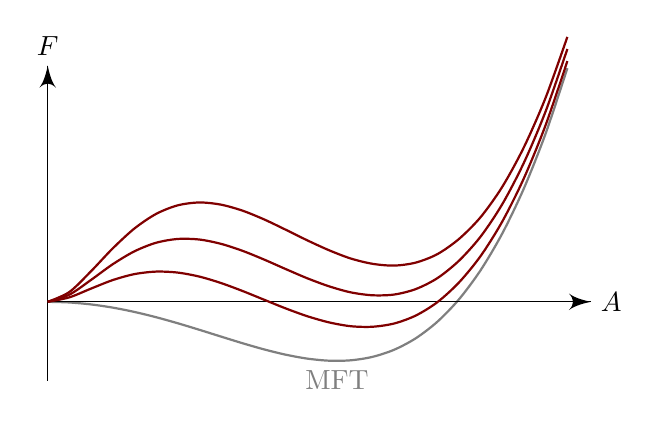
\begin{tikzpicture}[xscale=3]
    \draw [->] (0, 0) -- (2.3, 0) node [right] {$A$};
    \draw [->] (0, -1) -- (0, 3) node [above] {$F$};
    \draw [domain=0:2.2, opacity=0.5, thick] plot [smooth] (\x, {-(\x)^2 + (\x)^4/3});
    \draw [domain=0:2.2, mred, thick] plot [smooth] (\x, {(-1 + 10 * exp(-2.3 * \x)) * (\x)^2 - 5 * \x^3 * exp(-2.5 * \x) + (\x)^4/3});
    \draw [domain=0:2.2, mred, thick] plot [smooth] (\x, {(-1 + 15 * exp(-2.3 * \x)) * (\x)^2 - 5 * \x^3 * exp(-2.5 * \x) + (\x)^4/3});
    \draw [domain=0:2.2, mred, thick] plot [smooth] (\x, {(-1 + 20 * exp(-2.3 * \x)) * (\x)^2 - 5 * \x^3 * exp(-2.5 * \x) + (\x)^4/3});

    \node [opacity=0.5, below] at (1.2247, -0.75) {MFT};
  \end{tikzpicture}
\end{center}

We see that as $\tau$ decreases, the minimum discontinuously jumps from $A = 0$ to a finite value of $A$. Observe that mean field theory is approached at large $A$.

We can then plot the minimum value of $A$ as a function of $\tau$:
\begin{center}
  \begin{tikzpicture}
    \draw [domain=0:-4, opacity=0.5, thick, samples=50] plot [smooth] (\x, {1.8 * sqrt(- \x / 2)});
    \node [anchor = south west, opacity=0.5] at (-3.9, 2.514) {MFT};

    \draw [->] (-4, 0) -- (4, 0) node [right] {$\tau$};
    \draw [->] (0, 0) -- (0, 3) node [above] {$|A|$};

    \draw [mblue, thick] (3.9, 0) -- (-1.3, 0);
    \draw [dashed] (-1.3, 0) node [below] {$\tau_c$} -- (-1.3, 0.8) -- (0, 0.8) node [right] {$A_c$};
    \draw [mblue, thick] (-1.3, 0.8) .. controls (-2.2, 1.8) .. (-4, 2.53);

    \draw (-3, -0.08) node [below] {$\tau_H$} -- (-3, 0.08);
  \end{tikzpicture}
\end{center}
We have not calculated $A_c$ or $\tau_c$, but it can be done. We shall not do this, but we can state the result (Brazovskii, 1975):
\[
  \tau_c \simeq -(sb)^{2/3},\quad A_c \simeq s^{1/3} b^{-1/6}.
\]
It turns out the variational approach finally breaks down for $\tau < \tau_H \sim -s^{3/4} b^{1/2}$. We have $\tau_H \ll \tau_c$ if $b \ll \sqrt{s}$. The reason this breaks down is that at low enough temperatures, the fluctuations from the quartic terms become significant, and our Gaussian approximation falls apart.

To find $\tau_H$, we need to compute some leading corrections to $\tilde{F}$, as Brazovskii did. This is very rarely done. Most people don't bother to check how big the corrections to the approximation are. Thus, there is no reason to believe our theories are accurate. For example, if we do this for the Ising model, then everything goes wrong, because there is no regime where it is reasonable. So the self-consistent approach remains ad-hoc. However, in our case, it is asymptotically correct at small $b$.

\subsubsection*{Brazovskii transition with cubic term}
What happens when we have a cubic term? This would give an $A^3$ term at mean field level, which gives a discontinuous transition, but in a completely different way.

Let us plot a phase diagram with two parameters $\tau$ and $c$. In mean field theory, we get
\begin{center}
  \begin{tikzpicture}
    \draw [->] (-0.5, 0) -- (3, 0) node [right] {$c$};
    \draw [->] (0, -2) -- (0, 2) node [right] {$\tau$};

    \draw (0, 0) edge [bend right=10] (2.5, 1.8);
    \draw (0, 0) edge [bend left=10] (2.5, -1.8);
    \draw [fill=white] circle [radius=0.05];

    \node at (1, 1.5) {I};
    \node at (1, -1.5) {S};
    \node at (2, 0.5) {H};
  \end{tikzpicture}
\end{center}
where H is a hexagonal phase.

The self-consistent version instead looks like
\begin{center}
  \begin{tikzpicture}
    \draw [->] (-0.5, 0) -- (3, 0) node [right] {$c$};
    \draw [->] (0, -2) -- (0, 2) node [right] {$\tau$};

    \draw (0, -0.5) -- (1.7, -0.5) -- (3, 0.4);
    \draw (1.7, -0.5) -- (3, -1.4);

    \node at (1, 0.8) {I};
    \node at (1, -1.5) {S};
    \node at (2.5, -0.5) {H};

    \draw (1.7, -0.06) -- (1.7, 0.06) node [above] {\small$\tilde{c}$};
  \end{tikzpicture}
\end{center}
Here $c$ only matters above a threshold $\tilde{c}$.

The hexagonal phase looks like this:
\begin{center}
  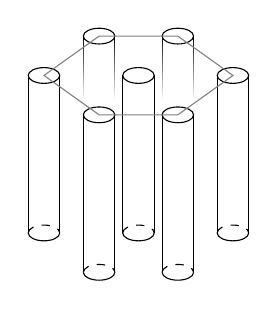
\begin{tikzpicture}
    \begin{scope}[shift={(0.3, 0)}]
      \draw ellipse (0.2 and 0.1);
      \draw (0.2, 0) -- (0.2, -2);
      \draw (-0.2, 0) -- (-0.2, -2);

      \draw (-0.2, -2) arc (180:360:0.2 and 0.1);
      \draw [dashed] (-0.2, -2) arc (180:0:0.2 and 0.1);
    \end{scope}
    \begin{scope}[shift={(1, -0.5)}]
      \draw ellipse (0.2 and 0.1);
      \draw (0.2, 0) -- (0.2, -2);
      \draw (-0.2, 0) -- (-0.2, -2);

      \draw (-0.2, -2) arc (180:360:0.2 and 0.1);
      \draw [dashed] (-0.2, -2) arc (180:0:0.2 and 0.1);
    \end{scope}
    \begin{scope}[shift={(2, -0.5)}]
      \draw ellipse (0.2 and 0.1);
      \draw (0.2, 0) -- (0.2, -2);
      \draw (-0.2, 0) -- (-0.2, -2);

      \draw (-0.2, -2) arc (180:360:0.2 and 0.1);
      \draw [dashed] (-0.2, -2) arc (180:0:0.2 and 0.1);
    \end{scope}
    \begin{scope}[shift={(2.7, 0)}]
      \draw ellipse (0.2 and 0.1);
      \draw (0.2, 0) -- (0.2, -2);
      \draw (-0.2, 0) -- (-0.2, -2);

      \draw (-0.2, -2) arc (180:360:0.2 and 0.1);
      \draw [dashed] (-0.2, -2) arc (180:0:0.2 and 0.1);
    \end{scope}

    \begin{scope}[shift={(1, 0.5)}]
      \draw ellipse (0.2 and 0.1);
      \draw [path fading=south] (0.2, 0) -- (0.2, -0.8);
      \draw [path fading=south] (-0.2, 0) -- (-0.2, -0.8);
    \end{scope}
    \begin{scope}[shift={(2, 0.5)}]
      \draw ellipse (0.2 and 0.1);
      \draw [path fading=south] (0.2, 0) -- (0.2, -0.8);
      \draw [path fading=south] (-0.2, 0) -- (-0.2, -0.8);
    \end{scope}
    \begin{scope}[shift={(1.5, 0)}]
      \draw ellipse (0.2 and 0.1);
      \draw (0.2, 0) -- (0.2, -2);
      \draw (-0.2, 0) -- (-0.2, -2);

      \draw (-0.2, -2) arc (180:360:0.2 and 0.1);
      \draw [dashed] (-0.2, -2) arc (180:0:0.2 and 0.1);
    \end{scope}

    \draw [gray](0.3, 0) -- (1, -0.5) -- (2, -0.5) -- (2.7, 0) -- (2, 0.5) -- (1, 0.5) -- cycle;
  \end{tikzpicture}
\end{center}
where each cylinder contains a high concentration of a fixed end of the molecule.

This is another liquid crystal, with two crystal directions and one fluid directions.

\section{Dynamics}
Ultimately, we are interested in field theories, but as a toy model, we start with a 1D particle. In the classical world, the action is given by
\[
  A = \int L\;\d t,\quad L = T - V.
\]
The equations of motion are
\[
  \frac{\delta A}{\delta x(t)} = \frac{\partial L}{\partial x} - \frac{\d}{\d t} \left(\frac{\partial L}{\partial x}\right) = 0.
\]
For example, if
\[
  L = \frac{1}{2} m\dot{x}^2 - V(x),
\]
then the equation of motion is
\[
  -\frac{\delta A}{\delta x(t)} = m\ddot{x} + V'(x) = 0.
\]
Note that this is deterministic. Also, in this system, the Lagrangian is invariant under time reversal, which we will assume to be the case in all our future examples. This is a consequence of the time reversal symmetry of microscopic laws.

We immerse the particle in a fluid bath, so that this is a colloid. We are not going to add all the new degrees of freedom from the individual fluid particles. Instead, we are going to simply add some new terms:
\begin{enumerate}
  \item We introduce damping, e.g.\ $F_D = - \zeta \dot{x}$.
  \item We introduce a noise $f$, with $\bra f \ket = 0$.
\end{enumerate}
We set $F_{BATH} = F_D + f$. Then we set our equation of motion to be
\[
  -\frac{\delta A}{\delta x} = - \zeta \dot{x} + f,
\]
the \term{Langevin equation}. The noise term is a sum of many independent contributions, so we will assume it is Gaussian. So the probability distribution of the realization of $f$ is
\[
  \P[f(t)] = \mathcal{N}_f \exp \left(- \frac{1}{\sigma^2} \int f(t)^2 \;\d t\right),
\]
where $\mathcal{N}_f$ is a normalization constant. This is called \term{white noise}, since
\[
  \bra f(t) f(t')\ket = \sigma^2 \delta(t - t').
\]

This is our assumption, which is one we will make throughout the course. We want to see how this translates to properties of the trajectory of the particle. To find the path probability (density) of an actual trajectory $x(t)$ between $(x_1, t_1)$ and $(x_2, t_2)$, consider the equation
\[
  f = \zeta \dot{x} - \frac{\delta A}{\delta x}.
\]
Then we have
\[
  \P_F[x(t)] \qeq \P[f] = \mathcal{N}_x \exp \left( -\frac{1}{2 \sigma^2} \int_{t_1}^{t_2} \left|\zeta \dot{x} - \frac{\delta A}{\delta x}\right|^2\;\d t\right).
\]
We might worry about the fact that we left out some Jacobian factors, but it turns out it doesn't matter.

How can we find the correct value of $\sigma$ to use? We are going to do something a bit strange now. We consider the backwards path, starting at $x_2$ and ending at $x_1$, given by $x(t_2 - t)$. On time reversal, the quantity $-\frac{\delta A}{\delta x}$ is unchanged by assumption of time reversibility. But we have $\dot{x} \mapsto -\dot{x}$ and $\d t \mapsto - \d t$. So the backwards probability is
\[
  \P_B[x(t)] = \mathcal{N}_x \exp \left( - \frac{1}{2\sigma^2}\int_{t_1}^{t_2} \left|-\zeta\dot{x} - \frac{\delta A}{\delta x}\right|^2\right)\;\d t.
\]
The only thing that changed is the sign in front of $- \zeta \dot{x}$.

We now construct
\begin{align*}
  \frac{\P_F[x(t)]}{\P_B[x(t)]} &= \frac{\exp \left(-\frac{1}{2\sigma^2} \int_{t_1}^{t_2} \left((\zeta \dot{x})^2 - 2 \zeta \dot{x} \frac{\delta A}{\delta x} + \left(\frac{\delta A}{\delta x}\right)^2\right)\;\d t\right)}{\exp \left(-\frac{1}{2\sigma^2} \int_{t_1}^{t_2} \left((\zeta \dot{x})^2 + 2 \zeta \dot{x} \frac{\delta A}{\delta x} + \left(\frac{\delta A}{\delta x}\right)^2\right)\;\d t\right)}\\
  &= \exp \left(-\frac{1}{2\sigma^2} \int_{t_1}^{t_2} \left(-4 \zeta \dot{x} \frac{\delta A}{\delta x}\right)\;\d t\right).
\end{align*}
To understand this integral, we go back to classical mechanics, and define Hamilton's function
\[
  H(x, \dot{x}) = \dot{x} \frac{\partial L}{\partial \dot{x}} - L.
\]
In our example, it is given by
\[
  H = \frac{1}{2} \dot{x}^2 + V(x).
\]
We have
\begin{align*}
  \frac{\d H}{\d t} &= \frac{\d}{\d t} \left(\dot{x} \frac{\partial L}{\partial \dot{x}}\right) - \frac{\d L}{\d t} \\
  &= \ddot{x} \frac{\partial L}{\partial \dot{x}} + \dot{x} \frac{\d}{\d t} \frac{\partial L}{\partial \dot{x}} - \left(\dot{x} \frac{\partial L}{\partial x} + \ddot{x} \frac{\partial L}{\partial \dot{x}}\right)\\
  &= \dot{x}\left(\frac{\d}{\d t} \left(\frac{\partial L}{\partial \dot{x}}\right) - \frac{\partial L}{\partial x}\right)\\
  &= - \dot{x} \frac{\delta A}{\delta x}.
\end{align*}
Therefore we get
\[
  \int_t^{t_2} \dot{x} \frac{\delta A}{\delta x(t)}\;\d t = - (H(x_2, \dot{x}_2) - H(x_1, \dot{x})) = - (H_2 - H_1).
\]
Therefore, a necessary and sufficient condition for
\[
  \frac{\P_F[x(t)]}{\P_B[x(t)]} \exp (-\beta(H_2 - H_1))\tag{$*$}
\]
for \emph{all} paths connecting $x_1, x_2$ is
\[
  \frac{4 \zeta}{2\sigma^2} = \beta,
\]
or equivalently
\[
  \sigma^2 = 2k_B T \zeta.
\]
The equation $(*)$ is \emph{required} by the \term{Principle of Detailed Balance} (\term{PDB}). Suppose we have microstates $A$, $B$. Then the probability of being in $B$ is $e^{-\beta H_A}$, and the probability of being in $B$ is $e^{-\beta H_B}$, up to a normalization by a constant factor.

We must observe the forward and backward events at equal rate in equilibrium. So it must be the case that
\[
  e^{-\beta H_A} \P(A \to B) = e^{-\beta H_B} \P(B \to A).
\]
The principle of detailed balance is a fundamental consequence of \emph{microscopic} reversibility. It is a symmetry, so coarse graining must respect it.

In the coarse grained world, suppose we have mesostates $A, B$, with probabilities $e^{-\beta F_A}$ and $e^{-\beta F_B}$, then we have an identical statement
\[
  e^{-\beta F_A} \P(A \to B) = e^{-\beta F_B} \P(B \to A).
\]
The summary is as follows: for a particle under a potential $V$, we have an equation
\[
  m\ddot{x} + V'(x) = - \zeta \dot{x} + f.
\]
The term $-\zeta \dot{x}$ gives an arrow of time en route to equilibrium, while the noise term resolves time reversal symmetry once equilibrium is reached. Requiring this fixes the variance, and we have
\[
  \bra f(t) f(t')\ket = \sigma^2 \delta(t - t') = 2 k_B T \zeta \delta(t - t').
\]
The statement
\[
  \sigma^2 = 2 k_B T \zeta
\]
is the simplest instance of the \term{fluctuation dissipation theorem}.

We write
\[
  f = \sqrt{2k_B T \zeta} \Lambda,
\]
where $\Lambda$ is a Gaussian process and
\[
  \bra \Lambda(t) \Lambda(t')\ket = \delta(t - t').
\]
We call this \term{unit white noise}\index{white noise!unit}.

\subsubsection*{Overdamped limit}
In the overdamped limit, we set $m = 0$. Then we have
\[
  \zeta \dot{x} = - \nabla V + \sqrt{2k_B T \zeta} \Lambda.
\]
Dividing by $\zeta$ and setting $\tilde{M} = \zeta^{-1}$, we get
\[
  \dot{x} = - \tilde{M} \nabla V + \sqrt{2k_B T \tilde{M}} \Lambda.
\]
This $\tilde{M}$ is the \term{mobility}, which is the velocity per unit force.

We want to get from Langevin to the diffusion equation. We may be interested in the probability
\[
  P(x, t) = \text{probability density at $x$ at time $t$}.
\]
We can look at the probability of moving by a distance $\Delta x$ in a time interval $\Delta t$. This is given by
\[
  P_{\Delta t}(\Delta x) = \mathcal{N} \exp \left(-\frac{1}{4 \zeta k_B T \Delta t} (\zeta \Delta x + \nabla V \Delta t)^2\right).
\]
Here we assume that $\zeta$ is not a function of position. We re-notate $\Delta x = u$. Then we have
\[
  \bra u\ket = - \frac{\nabla V}{\zeta} \Delta t,\quad \bra u^2\ket - \bra u\ket^2 = \frac{2k_B T}{\zeta} \Delta t + O(\Delta t^2).
\]
We write
\[
  W(u, x) = P_{\Delta t}(u),
\]
the probability of moving by $u$ in $\Delta t$ starting at $x$. Then we have
\[
  \int W(u, x) = 1.
\]
We can find a \emph{deterministic} equation for $P(x, t)$. We have
\[
  P(x, t + \Delta t) = \int P(x - u, t) W(u, x - u)\;\d u.
\]
Taylor expanding the integrand gives
\[
  \left(P - u \nabla P + \frac{1}{2} u^2 \nabla^2 P\right)\left(W(u, x) - u \nabla W + \frac{1}{2} u^2 \nabla^2 W\right),
\]
where all the gradients act on $x$, not $u$. We integrate over $u$ to get
\[
  P(x, t + \Delta t) = P(x, t) - \bra u \ket \nabla P + \frac{1}{2} \bra u^2\ket \nabla^2 P + P \nabla \bra u\ket,
\]
using that
\begin{align*}
  \int W \;\d u &= 1\\
  \int u W \;\d u&= \bra u\ket\\
  \int u^2 W \;\d u &= \bra u^2\ket = \frac{2k_B T}{\zeta} + O(\Delta t^2)\\
  \int u \nabla_x W\;\d u &= \nabla_x \bra u\ket_W = - \frac{\nabla^2 V}{\zeta}\Delta t.
\end{align*}
Gathering terms, we have
\[
  P(x, t + \Delta t) = P(x, t) - \bra u\ket_W \nabla P + \frac{1}{2} \bra u^2\ket_W \nabla^2 P - P \nabla \bra u\ket_W + \cdots,
\]
and substituting in the above results gives
\[
  \dot{P}(x, t) \Delta t = \left(\frac{\nabla V}{\zeta} \nabla P + \frac{k_B T}{\zeta} \nabla^2 P + \frac{1}{\zeta} P \nabla^2 V \right)\Delta t.
\]
Dividing by $\Delta t$, we get
\begin{align*}
  \dot{P} &= \frac{k_B T}{\zeta} \nabla^2 P + \frac{1}{\zeta} \nabla(P \nabla V)\\
  &= D \nabla^2 P + \tilde{M} \nabla(P \nabla V),
\end{align*}
where $D = \frac{k_B T}{\zeta}$ is the \term{diffusivity} and $\tilde{M} = \frac{D}{k_B T} = \frac{1}{\zeta}$ is the \term{mobility}.

Putting a subscript one to emphasize that we are working with one particle, the structure of this is
\begin{align*}
  \dot{P}_1 &= - \nabla \cdot \mathbf{J}_1\\
  \mathbf{J}_1 &= -P_1 D \nabla (\log P_1 + \beta V)\\
  &= -P_1 \tilde{M} \nabla \mu(x),
\end{align*}
where
\[
  \mu = k_B T \log P_1 + V
\]
is the chemical potential of a particle in $V(x)$. Observe that
\begin{itemize}
  \item This is deterministic for $P_1$.
  \item This has the same information as the Langevin equation, which gives the statistics for paths $x(t)$.
  \item This was ``derived'' for a constant $\zeta$, independent of position. However, the equations in the final form turn out to be correct even for $\zeta = \zeta(x)$ as long as the temperature is constant, i.e.\ $\tilde{M} = \tilde{M}(x) = \frac{D(x)}{k_B T}$. In this case, the Langevin equation says
    \[
      \dot{x} = - \tilde{M}(x) \nabla V + \sqrt{2 D(x)} \Lambda.
    \]
    The multiplicative noise term is problematic. To understand this equation with a noise that depends on the stochastically varying coordinate, we need advanced stochastic calculus (It\^o/Stratonovich).
\end{itemize}
In this course, we avoid multiplicative noise.

\subsection{From one particle to many}
Suppose we have $N$ non-interacting colloids in $V(x)$. What we are interested in is some kind of coarse grained density $\rho(x, t)$. If there are non-interacting, we can simply multiply together these distributions, and we have
\[
  \bra \rho\ket = NP,\quad \bra \dot{\rho}\ket = N \dot{P}_1.
\]
If this is the case, then we have
\[
  \dot{\rho} = - \nabla \cdot \mathbf{J},
\]
where
\[
  \bra \mathbf{J}\ket = - \rho \tilde{M} \nabla \mu,\quad \mu = k_B T \log \rho + V(x).
\]
With interactions, we set $\mu = \frac{\delta F}{\delta \rho}$, and see what happens. This is phenomenological, but well-motivated.

But setting $\mathbf{J} = \bra \mathbf{J}\ket$ neglects fluctuations in particle current. These equations only give us a \emph{hydrodynamic level} (deterministic) equation of motion for $\rho$. This evolves to a mean field solution, where $\mu$ becomes a constant and $F[\rho]$ goes to its minimum at fixed $N = \int \rho(\mathbf{r}, t) \;\d \mathbf{r}$.

Contrast $P_1$, the probability density for $1$ particle, which \emph{does} have a deterministic equation, which is equivalent to Langevin for paths; with $\rho$, a particle density, which is \emph{not} a probability density, and this is a fluctuating quantity. We need a Langevin equation for $\rho$ whose average will be what we have above.

Instead of the mean field solution, we require the Boltzmann distribution, namely the steady state probability distribution is
\[
  P_{ss}[\rho] = \mathcal{N} e^{-\beta F[\rho]}.
\]
This requires
\[
  \dot{\rho} = - \nabla \cdot \mathbf{J},
\]
which is always the case since $\rho$ is conserved, but now
\[
  \mathbf{J} = - \rho \tilde{M} \nabla \mu + \mathbf{j},
\]
where $\mathbf{j}$ is a \term{noise current}. This is the Langevin equation for a fluctuating field $\rho(\mathbf{r}, t)$.

We can fix the distribution of $\mathbf{j}$ by requiring detailed balance as before. We will implement this for a constant $M = \rho \tilde{M}$. We call this the \term{collective mobility} This is what we have to do to avoid having multiplicative noise in our system. While this doesn't seem very physical, this makes more sense, for example, when we are looking at fluctuations about a fixed density.

As before, we assume $\mathbf{j}(r, t)$ is Gaussian white noise, so
\[
  \P[\mathbf{j}(\mathbf{r}, t)] = \mathcal{N} \exp \left(-\frac{1}{2\sigma^2} \int_{t_1}^{t_2} \d t\int \d \mathbf{r} |\mathbf{j}(\mathbf{r}, t)|^2\right).
\]
This corresponds to
\[
  \bra j_k (\mathbf{r}, t)j_\ell(\mathbf{r}', t')\ket = \sigma^2 \delta_{k\ell} \delta(\mathbf{r} - \mathbf{r}') \delta(t - t').
\]
We now repeat the detailed balance argument to find $\sigma^2$. We start from
\[
  \mathbf{J} + M \nabla \mu = \mathbf{j}.
\]
Using $F$ to mean forward path, we have
\[
  \P_F[\mathbf{J}(\mathbf{r}, t)] = \mathcal{N} \exp \left(-\frac{1}{2\sigma^2} \int_{t_1}^{t_2} \d t \int \d \mathbf{r} \; |\mathbf{J} + M \nabla \mu|^2 \right),
\]
where
\[
  \mu = \frac{\delta F[\rho]}{\delta \rho}.
\]
We consider the backwards part and get
\[
  \P_B[\mathbf{J}(\mathbf{r}, t)] = \mathcal{N} \exp \left(-\frac{1}{2\sigma^2} \int_{t_1}^{t_2} \d t \int \d \mathbf{r} \; |-\mathbf{J} + M \nabla \mu|^2 \right),
\]
Then
\[
  \log \frac{\P_F}{\P_B} = - \frac{2M}{\sigma^2} \int_{t_1}^{t_2} \d t \int \d \mathbf{r} \mathbf{J} \cdot \nabla \mu.
\]
This is fixed by the principle of detailed balance.

We integrate by parts in space to write
\[
  \int \d \mathbf{r}\; \mathbf{J} \cdot \nabla \mu = - \int \d \mathbf{r}\; (\nabla \cdot \mathbf{J}) \mu = \int \d \mathbf{r} \left(\dot{\rho} \frac{\delta F}{\delta \rho}\right) = \frac{\d F[\rho]}{\d t}.
\]
So we get
\[
  \log \frac{\P_F}{\P_B} = - \frac{2M}{\sigma^2} (F_2 - F_1).
\]
So we need
\[
  \frac{2M}{\sigma^2} = \beta,
\]
or equivalently
\[
  \sigma^2 = 2k_B T M.
\]
So our final many-body Langevin equation is
\begin{align*}
  \dot{\rho} &= - \nabla \cdot \mathbf{J}\\
  \mathbf{J} &= - M \nabla \left(\frac{\delta F}{\delta \rho}\right) + \sqrt{2k_B T M} \Lambda,
\end{align*}
where $\Lambda$ is spatiotemporal unit white noise. A constant $M$ avoids multiplicative white noise.

In general, we get the same structure for any other diffusive system, such as $\phi(\mathbf{r}, t)$ in a binary fluid.
\subsubsection*{Langevin to Fokker--Planck}
For one particle, we had the Langevin equation
\[
  \dot{x} = - \tilde{M} \nabla V + \sqrt{2k_B T \tilde{M}} \Lambda,
\]
and this became the equation
\begin{align*}
  \dot{P} &= - \nabla \cdot \mathbf{J}\\
  \mathbf{J} &= -P \tilde{M} \nabla \mu\\
  \mu &= k_B T \log P + V(x).
\end{align*}
We then write this as
\[
  \dot{P} = \nabla \cdot \left(\tilde{M} k_B T \left(\nabla + \beta \nabla V\right)P\right),
\]
where $P(x, t)$ is the time dependent probability density for $x$.

A similar equation can be derived for the multi-particle case, which we will write down but not derive. We replace $x(t)$ with $\rho(\mathbf{r}, t)$, and we replace $P(x, t)$ with $P[\rho(\mathbf{r}); t]$. We then replace $\nabla$ with $\frac{\delta}{\delta \rho(\mathbf{r})}$. So the Fokker--Planck equation becomes
\[
  \dot{P}[\rho(t); t] = \int \d \mathbf{r} \; \frac{\delta}{\delta \rho} \left(k_B T \nabla \cdot \tilde{M} \nabla \left(\frac{\delta}{\delta \rho} + \beta \frac{\delta F}{\delta \rho}\right)P\right).
\]
This is the \term{Fokker--Planck equation} for fields $\rho$.

As one can imagine, it is not very easy to solve. Note that in both cases, the quantities $\nabla + \beta \nabla V$ and $\frac{\delta}{\delta \rho} + \beta \frac{\delta F}{\delta \rho}$ annihilate the Boltzmann distribution. So the Boltzmann distribution is invariant.

The advantage of the Langevin equation is that it is easy to understand the mean field theory/deterministic limit $\rho = \rho_{hydro}(\mathbf{r}, t)$. However, it is difficult to work with multiplicative noise. In the Fokker--Planck equation, multiplicative noise is okay, but the deterministic limit may be singular. Schematically, we have
\[
  P[\rho(\mathbf{r}), t] = \delta(\rho(\mathbf{r}, t) - \rho_{hydro}(\mathbf{r}, t)).
\]
In this course, we take the compromise and use the Langevin equation with constant $M$.

\section{Model B}
We now wish to understand the dynamics of a particular model of binary fluid --- Model B. This is a pure diffusion system with no fluid flow. This has a scalar composition field $\phi(\mathbf{r})$, and we have
\begin{align*}
  \dot{\phi} &= - \nabla \cdot \mathbf{J}\\
  \mathbf{J} &= - M \nabla \mu + \sqrt{2k_B TM} \boldsymbol \Lambda\\
  \mu &= \frac{\delta F}{\delta \phi}.
\end{align*}
We choose the same Landau--Ginzburg free energy as we always have,
\[
  F[\phi] = \int \left(\underbrace{\frac{a}{2} \phi^2 + \frac{b}{4}\phi^4}_f + \frac{\kappa}{2} (\nabla \phi)^2\right)\;\d \mathbf{r}.
\]
We then have
\[
  \mu = a \phi + b \phi^3 - \kappa \nabla^2 \phi.
\]
The mean field theory for equilibrium has the usual picture
\begin{center}
  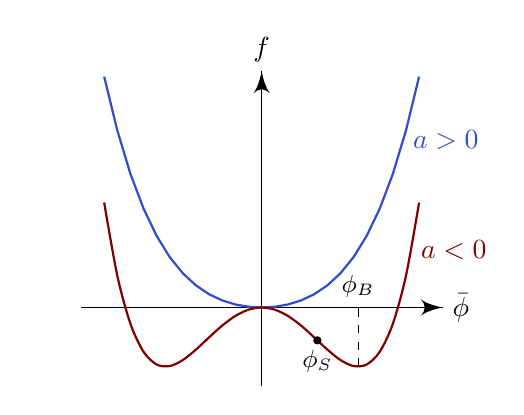
\begin{tikzpicture}
    \draw [->] (-2.3, 0) -- (2.3, 0) node [right] {$\bar{\phi}$};
    \draw [->] (0, -1) -- (0, 3) node [above] {$f$};
    \draw [domain=-2:2, mblue, thick] plot (\x, {(\x)^2/3 + (\x)^4/10});
    \draw [domain=-2:2, mred, thick] plot [smooth] (\x, {-(\x)^2 + (\x)^4/3});

    \node [right, mblue] at (1.8, 2.13) {$a > 0$};
    \node [right, mred] at (1.9, 0.734) {$a < 0$};
    \node [left, white] at (-1.8, 2.13) {$a > 0$};
    \node [left, white] at (-1.9, 0.734) {$a < 0$};

    \draw [dashed] (1.2247, -0.75) -- (1.2247, 0) node [above] {\small$\phi_B$};
    \draw (0.707, -0.417) node [below] {\small$\phi_S$} node [circ] {};
  \end{tikzpicture}
\end{center}
Here $\pm \phi_S$ are the spinodals, where the second derivative changes sign. This gives the phase diagram
\begin{center}
  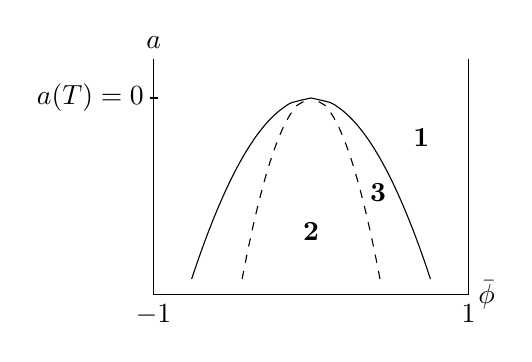
\begin{tikzpicture}
    \draw (-2, 3) node [above] {$a$} -- (-2, 0) node [below] {$-1$} -- (2, 0) node [below] {$1$} node [right] {$\bar \phi$} -- (2, 3);
    \node [left] at (-2, 2.5) {$a(T) = 0$};

    \draw [domain=2.5:0.2, samples=40] plot [smooth] ({sqrt (2.5 - \x)}, \x);
    \draw [domain=2.5:0.2, samples=40] plot [smooth] ({-sqrt (2.5 - \x)}, \x);

    \draw [dashed, domain=0.2:2.5] plot [smooth] ({sqrt ((2.5 - \x)/3)}, \x);
    \draw [dashed, domain=0.2:2.5] plot [smooth] ({-sqrt ((2.5 - \x)/3)}, \x);
    \draw (-2.05, 2.5) -- (-1.95, 2.5);

    \node at (1.4, 2) {$\mathbf{1}$};
    \node at (0.85, 1.3) {$\mathbf{3}$};
    \node at (0, 0.8) {$\mathbf{2}$};
  \end{tikzpicture}
\end{center}
Here $\bar{\phi}$ is the global composition, which is a control variable.
\begin{itemize}
  \item In (1), we have $|\bar{\phi}| > \phi_B$. Then have a uniform phase which is globally stable.
  \item In (2), we have $|\bar{\phi}| < \phi_S$. Then $f''(\phi) < 0$ implies local instability. This is \term{spinodal behaviour}.
  \item In (3), we have $\phi_S < |\bar{\phi}| < \phi_B$. A uniform phase is locally stable, but not globally. To reach phase separated, we need nucleation and growth. This will require the contribution of noise.
\end{itemize}
We now study these in detail.
\subsubsection*{Regime 1}
First consider the regime (1). Consider small fluctuations about $\phi(r) = \bar{\phi}$, so we write $\phi = \bar{\phi} + \tilde{\phi}(\mathbf{r})$. We can then write
\[
  \mu = \frac{\delta F}{\delta \phi} = \frac{\partial f}{\partial \phi} - \kappa \nabla^2 \phi = f'(\bar{\phi}) + \tilde{\phi} f''(\bar{\phi}) - \kappa \nabla^2 \tilde{\phi}.
\]
Note that the first term is a constant. We then have
\begin{align*}
  \dot{\phi} &= - \nabla \cdot \mathbf{J}\\
  \mathbf{J} &= -M \nabla [f''\tilde{\phi} - \kappa \nabla^2 \tilde{\phi}] + \sqrt{2k_B T M} \boldsymbol\Lambda.
\end{align*}
We drop the tildes and take the Fourier transform to get
\[
  \dot{\phi}_{\mathbf{q}} = - M q^2 (f'' + \kappa q^2)\phi_{\mathbf{q}} + i\mathbf{q} \cdot \sqrt{2k_B TM} \boldsymbol\Lambda_{\mathbf{q}}.
\]
Compare this with an overdamped particle in a simple harmonic oscillator,
\[
  V = \frac{1}{2} \kappa x^2,
\]
where we have
\[
  \dot{x} = - \tilde{M} \kappa x + \sqrt{2k_B T \tilde{M}} \Lambda.
\]
Refer to example sheet 2 problems 8 and 9, where we computed
\[
  S(q, t) \equiv \bra \phi_\mathbf{q}(0) \phi_{-\mathbf{q}} (t)\ket = S(q) e^{-r(q) t},
\]
where
\[
  r(q) = Mq^2(f'' + \kappa q^2).
\]
Here $s(q)$ is the equilibrium equal time static correlator, which is
\[
  \frac{k_B T}{f'' + \kappa q^2}.
\]
This \term{$S(\mathbf{q}, t)$} is called the \term{dynamic structure factor}, which can be measured by light scattering.
\subsubsection*{Regime 2}
In the second regime, we have the same equation
\[
  \dot{\phi}_{\mathbf{q}} = - M q^2 (f'' + \kappa q^2)\phi_\mathbf{q} + i\mathbf{q} \cdot \sqrt{2k_B TM} \boldsymbol\Lambda_{\mathbf{q}}.
\]
but crucially, $f''(\bar{\phi}) < 0$. So when $q^2 < - \frac{f''}{\kappa}$, the system is unstable.

We first ignore the noise by averaging the equation to get
\[
  \bra \dot{\phi}_\mathbf{q}\ket = - r(q) \bra \phi_q\ket.
\]
Observe that $-r(q) > 0$ at $q < \sqrt{\frac{-f''}{\kappa}}$. This is the growth rate of the perturbations. So if we have a noisy initial state $\phi_\mathbf{q}(0)$, then we have
\[
  \bra \phi_\mathbf{q}(t)\ket = \phi_\mathbf{q}(0) e^{-r(q)t}.
\]
The is an amplification of the initial noise. Because of this, the noise becomes irrelevant at late times.

We can plot our $r(q)$ as follows:
\begin{center}
  \begin{tikzpicture}
    \draw [->] (0, 0) -- (4, 0) node [right] {$q$};
    \draw [->] (0, -1.3) -- (0, 3) node [above] {$r(q)$};
    \draw [domain=0:3.8, thick, mblue] plot [smooth] (\x, {\x^2 * (-2 + \x^2/5) / 5});

    \draw [dashed] (2.236, -1) -- (2.236, 0) node [above] {$q^*$};
  \end{tikzpicture}
\end{center}
the maximally unstable mode $q^*$ is given by the solution to $r'(q^*) = 0$, which we can easily check to be given by
\[
  q^* = \sqrt{\frac{-f''}{2\kappa}}.
\]
Now consider the equal time \term{non-equilibrium structure factor}\index{$S_\mathbf{q}(t)$}
\[
  S_\mathbf{q}(t) = \bra \phi_\mathbf{q}(t) \phi_{-\mathbf{q}}(t)\ket \sim S_\mathbf{q}(0) e^{-2r(q) t}.
\]
As time evolves, this gets more and more peaked around $q = q^*$:
\begin{center}
  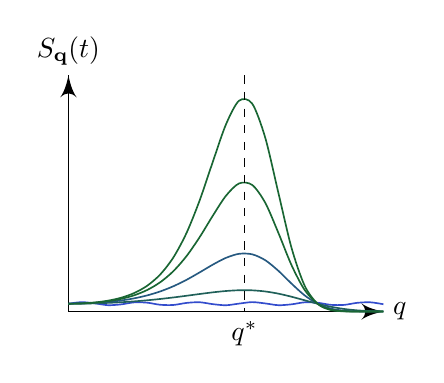
\begin{tikzpicture}
    \draw [->] (0, 0) -- (4, 0) node [right] {$q$};
    \draw [->] (0, 0) -- (0, 3) node [above] {$S_\mathbf{q}(t)$};

    \draw[domain=0:4, mblue, semithick] plot [smooth] (\x, {0.1 + 0.02 * sin(500 * \x)});
    \draw[domain=0:4, mblue!25!mgreen, semithick] plot [smooth] (\x, {0.1 * e^(- \x^2 * (-2 + \x^2/5) / 5)});
    \draw[domain=0:4, mblue!50!mgreen, semithick] plot [smooth] (\x, {0.1 * e^(-2* \x^2 * (-2 + \x^2/5) / 5)});
    \draw[domain=0:4, mgreen!75!mgreen, semithick] plot [smooth] (\x, {0.1 * e^(-2.8* \x^2 * (-2 + \x^2/5) / 5)});
    \draw[domain=0:4, mgreen, semithick] plot [smooth] (\x, {0.1 * e^(-3.3* \x^2 * (-2 + \x^2/5) / 5)});
    \draw [dashed] (2.236, 3) -- (2.236, 0) node [below] {$q^*$};
  \end{tikzpicture}
\end{center}
So we see a growth of random structure with scale $L \sim \pi/q^*$. This process is called \term{spinodal decomposition}.
\begin{center}
  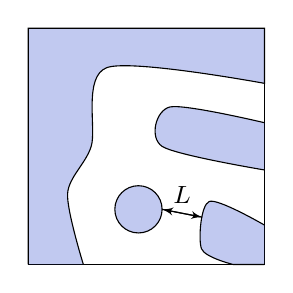
\begin{tikzpicture}
    \draw (0, 0) rectangle (3, 3);
    \draw [fill=mblue, fill opacity=0.3] plot [smooth] coordinates {(0.7, 0) (0.5, 0.9) (0.8, 1.5) (1, 2.5) (3, 2.3)} -- (3, 3) -- (0, 3) -- (0, 0);

    \draw [fill=mblue, fill opacity=0.3] (1.4, 0.7) circle [radius=0.3];

    \draw [fill=mblue, fill opacity=0.3] plot[smooth] coordinates {(3, 1.8) (1.8, 2) (1.7, 1.5) (3, 1.2)};

    \draw [fill=mblue, fill opacity=0.3] plot[smooth] coordinates {(3, 0.5) (2.3, 0.8) (2.2, 0.2) (2.6, 0)} -- (3, 0);

    \draw [-latex'] (1.7, 0.7) -- (2.21, 0.6) node [pos=0.5, above] {\small $L$};
    \draw [-latex'] (2.21, 0.6) -- (1.7, 0.7);
  \end{tikzpicture}
\end{center}
At intermediate $t$, the quartic terms are going to kick in. An informal use of variational theory says we should replace $f''$ by $\bar{f}''$.
\[
  \bar{f}'' = f'' + \frac{3b}{(2\pi)^4} \int^{q_{max}} S_q(t) \;\d^d \mathbf{q}.
\]
This says $\bar{f}''$ is less negative as the fluctuations grow. So
\[
  q^* = \sqrt{\frac{-\bar{f}''}{2k}},
\]
and this moves to a smaller $q$. So $L(t) \sim \pi/q^*(t)$ starts decreasing. This is called \term{domain growth}.

In the late stages, we have regions of $\phi \approx \pm \phi_B$, so it is almost in equilibrium locally. We are well away from the exponential growth regime, and the driving force for domain growth is the reduction of interfacial area. We can estimate the free energy (per unit volume) as
\[
  \frac{F}{V} = \frac{\sigma A(t)}{V},
\]
where $A(t)$ is the area of the interface. So by dimensional analysis, this is $\sim \sigma/L(t)$. We have calculated the interfacial surface tension $\sigma$ before to be
\[
  \sigma = \left(\frac{-8\kappa a^3}{9b^2}\right)^{1/2},
\]
but it doesn't really matter what this is. The ultimate configuration with minimal surface area is when we have complete phase separation. The result is that
\[
  L(t) \sim \left(\frac{M_\sigma}{\phi_B} t\right)^{1/3}.
\]
We will not derive this yet, because this result is shared with the late time behaviour of the third regime, and we will discuss this at that point.

\subsubsection*{Regime 3}
Finally, consider the third regime. Suppose we have $\bar{\phi} = -\phi_B + \delta$, where $\delta$ is small. This is locally stable, so $r(q) > 0$ for all $q$. But this is globally unstable, and we prefer phase separation. Only noise can overcome the \term{nucleation barrier}. But what is the path? In other words, what is the typical way a uniform phase manages to go into phase separation?

Formally, we can inspect the path probabilities
\[
  \P[\phi(\mathbf{r}, t)] = \mathcal{N} \exp \left(-\frac{\beta}{4M} \int |\mathbf{J} + M \nabla \mu|^2 \;\d \mathbf{r} \;\d t\right)
\]
given by the Langevin equation. We seek to find the most likely trajectory from the initial to the final state. If one is a field theorist, then this is called the \term{instanton path}, and in statistical physics, this is called \term{large deviation theory}. Instead of doing this, we use our physical intuition to guide ourselves.

Heuristically, we expect that if we start with a uniform phase $\phi = -\phi_B + \delta$, then at some point, there will be some random small droplet with $\phi = +\phi_B$ of radius $R$. We then hope that $R$ increases until we have full phase separation. The key question is --- how unlikely is this process?
\begin{center}
  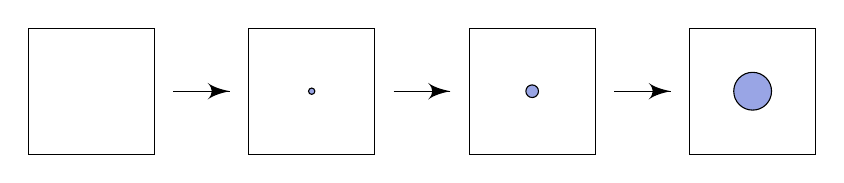
\begin{tikzpicture}[scale=0.8]
    \draw (0, 0) rectangle (2, 2);
    \draw [->] (2.3, 1) -- (3.2, 1);
    \begin{scope}[shift={(3.5, 0)}]
      \draw (0, 0) rectangle (2, 2);
      \draw [fill=mblue, fill opacity=0.5] (1, 1) circle [radius=0.05];
      \draw [->] (2.3, 1) -- (3.2, 1);
    \end{scope}

    \begin{scope}[shift={(7, 0)}]
      \draw (0, 0) rectangle (2, 2);
      \draw [fill=mblue, fill opacity=0.5] (1, 1) circle [radius=0.1];
      \draw [->] (2.3, 1) -- (3.2, 1);
    \end{scope}

    \begin{scope}[shift={(10.5, 0)}]
      \draw (0, 0) rectangle (2, 2);
      \draw [fill=mblue, fill opacity=0.5] (1, 1) circle [radius=0.3];
    \end{scope}
  \end{tikzpicture}
\end{center}
The idea is to consider the cost of having a droplet of radius $R$. First consider the cost of having an interface, which is $4 \pi \sigma R^2$. However, we also want a droplet with large volume, so we get a cubic term $\sim -R^3$ with negative contribution. If we add these two together, we get a barrier:
\begin{center}
  \begin{tikzpicture}
    \draw [->] (0, 0) -- (4, 0) node [right] {$R$};
    \draw [->] (0, -1.8) -- (0, 2.5) node [above] {$F(R)$};

    \draw [domain=0:3.7, mblue, semithick] plot [smooth] (\x, {3*(\x^2/3 -\x^3/10)});

    \draw [dashed] (2.222, 1.6461) -- (2.222, 0) node [below] {$R^*$};
    \draw [dashed] (2.222, 1.6461) -- (0, 1.6461) node [left] {$F^*$};
  \end{tikzpicture}
\end{center}
Here $R^*$ is the critical radius, and $F^*$ is the free energy barrier. The noise-induced rate, which is the rate of getting over the barrier, is $\sim e^{-\beta F^*}$.

\subsubsection*{Droplet in equilibrium}
Consider the equilibrium of a droplet with its ``vapour''. If $\phi$ is just close to $-\phi_B$, then there will be a small spherical droplet of $+\phi_B$ of radius $R$, and the rest being at $-\phi_B$. So we have two bulk phases separated by a curved surface (contrast this to the case where $\phi = 0$, where we would have a horizontal interface).
\begin{center}
  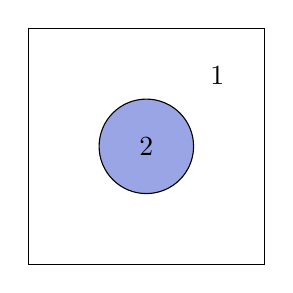
\begin{tikzpicture}
    \draw (0, 0) rectangle (3, 3);
    \draw [fill=mblue, fill opacity=0.5] (1.5, 1.5) circle [radius=0.6];
    \node at (1.5, 1.5) {$2$};
    \node at (2.4, 2.4) {$1$};
  \end{tikzpicture}
\end{center}
Within each region $1$ and $2$, our $\phi$ is constant, so the term that contributes to the free energy is
\[
  f (\phi) = \frac{a}{2} \phi^2 + \frac{b}{4} \phi^4.
\]
We would expect $1$ and $2$ to respectively be located at
\begin{center}
  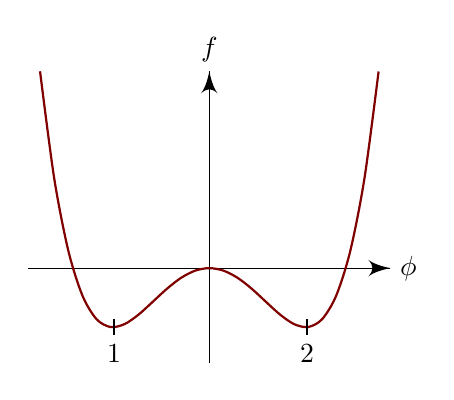
\begin{tikzpicture}
    \draw [->] (-2.3, 0) -- (2.3, 0) node [right] {$\phi$};
    \draw [->] (0, -1.2) -- (0, 2.5) node [above] {$f$};
    \draw [domain=-2.15:2.15, mred, thick] plot [smooth] (\x, {-(\x)^2 + (\x)^4/3});

    \draw (-1.21, -0.65) -- (-1.21, -0.85) node [below] {$1$};
    \draw (1.24, -0.65) -- (1.24, -0.85) node [below] {$2$};
  \end{tikzpicture}
\end{center}
Note that when we have a spherical interface, $1$ and $2$ are not exactly at $\pm \phi_B$. To understand this, Consider the \term{bulk chemical potential}
\[
  \mu = \frac{\partial f}{\partial \phi},
\]
 The thermodynamic pressure is then
\[
  \Pi = \mu \phi - f.
\]
If we have a flat interface, which we can think of as the limit $R \to \infty$, then we require
\[
  \mu_1^{bulk} = \mu_2^{bulk},\quad \Pi_1^{bulk} = \Pi_2^{bulk}.
\]
This means the points 1, 2 have a common tangent
\begin{center}
  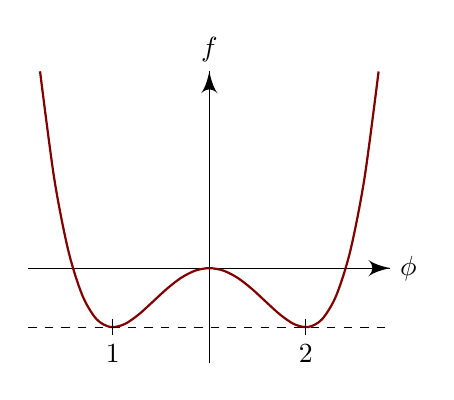
\begin{tikzpicture}
    \draw [->] (-2.3, 0) -- (2.3, 0) node [right] {$\phi$};
    \draw [->] (0, -1.2) -- (0, 2.5) node [above] {$f$};
    \draw [domain=-2.15:2.15, mred, thick] plot [smooth] (\x, {-(\x)^2 + (\x)^4/3});

    \draw (-1.2247, -0.65) -- (-1.2247, -0.85) node [below] {$1$};
    \draw (1.2247, -0.65) -- (1.2247, -0.85) node [below] {$2$};

    \draw [dashed] (-2.3, -0.75) -- (2.3, -0.75);
  \end{tikzpicture}
\end{center}

If we have a droplet, then there is surface tension. Consider an imaginary interface between the upper and lower interface. Then the pressure difference tries to move the upper hemisphere up, and contributes a force of $(\Pi_2 - \Pi_1) \pi R^2$, while the interfacial tension pulls the boundary down by $2\pi R \sigma$. So we require
\[
  \Pi_2 = \Pi_1 + \frac{\sigma}{R}(d - 1)
\]
in $d$ dimensions. This is called the \term{Laplace pressure}.

In the static equilibrium, we have $\mathbf{J} = 0$. So $\nabla \mu = 0$, and so $\mu_1 = \mu_2$. Thus, we have $\psi_1 = -\phi_B + \delta_1 $ and $\psi_2 = +\phi_B + \delta_2$, such that $f$ has the same slope at $\phi_1$ and $\phi_2$.
\begin{center}
  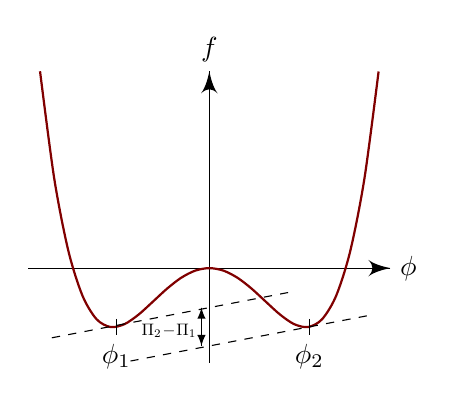
\begin{tikzpicture}
    \draw [->] (-2.3, 0) -- (2.3, 0) node [right] {$\phi$};
    \draw [->] (0, -1.2) -- (0, 2.5) node [above] {$f$};
    \draw [domain=-2.15:2.15, mred, thick] plot [smooth] (\x, {-(\x)^2 + (\x)^4/3});

    \draw (-1.18, -0.646) -- (-1.18, -0.846) node [below] {$\phi_1$};
    \draw (1.27, -0.6458) -- (1.27, -0.8458) node [below] {$\phi_2$};

    \draw [dashed] (2, -0.6062) -- (-1, -1.1797);
    \draw [dashed] (-2, -0.88496) -- (1, -0.31);

    \draw [-latex] (-0.1, -0.988533) -- (-0.1, -0.501653) node [pos=0.4, left] {\scalebox{0.6}{$\Pi_2\!-\!\Pi_1$}\!};
    \draw [-latex] (-0.1, -0.501653) -- (-0.1, -0.988533);
  \end{tikzpicture}
\end{center}

For large $R$, we expect $\delta$ to be small. So we can approximate
\begin{align*}
  f_1 &= f(-\phi_B + \delta_1) \approx \frac{1}{2} f''(-\phi_B) + \delta_1^2 + f(-\phi_B)\\
  f_2 &= f(+\phi_B + \delta_2) \approx \frac{1}{2} f''(+\phi_B) + \delta_1^2 + f(+\phi_B).
\end{align*}
So $\mu_i = \alpha \delta_i$, where $\alpha = f''(\pm\phi_B)$. So we find that up to first order, $\delta_1 = \delta_2$.

To compute $\delta$, we compute
\[
  \Pi_1 = \mu_1\phi_1 - f_1 = -\alpha \delta \phi_B.
\]
Similarly, we have $\Pi_2 = +\alpha \delta \phi_B$. So
\[
  \Pi_1 - \Pi_2 = -2\alpha \phi_B \delta.
\]
Since this equals $-(d - 1)\frac{\sigma}{R}$, we have
\[
  \delta = \frac{1}{2\alpha \phi_B}(d - 1) \frac{\sigma}{R}.
\]

\subsubsection*{Hydrodynamic level mean field theory for multiple droplet}
We now want to understand what happens when we have multiple droplets. The way multiple droplets interact is that once we have a droplet of large $\phi$, then the average $\phi$ outside of the droplet will decrease. So to begin understanding this scenario, we first see how a droplet reacts when the relative density of the outside bath is not what it expects.

So suppose we have a (3D) droplet of radius $R$ inside a bath with $\phi = - \phi_B + \varepsilon$. This $\varepsilon$ is called the \term{supersaturation}. Note that to have a droplet of radius $R$, the value of $\phi$ inside and immediately outside the droplet must be $\pm \phi_B + \delta$, where $\delta = \delta(R)$ is the value we previously computed.
Outside of the droplet, the value of $\phi$ will slowly decay to $\varepsilon$. Thus, outside of the droplet, we write
\[
  \phi(\mathbf{r}) = -\phi_B+ \tilde{\phi}(\mathbf{r}),
\]
where $\tilde{\phi}(\infty) = \varepsilon$ and $\tilde{\phi}(R^+) = \delta$.

In this situation, unless $\delta$ happens to be $\varepsilon$, we have a gradient of $\phi$, hence a gradient of chemical potential, hence a flux. Again in Model B, we have
\[
  \dot{\phi} = - \nabla \cdot \mathbf{J},\quad \mathbf{J} = -M \nabla \mu = -M \alpha \nabla \tilde{\phi}(\mathbf{r}),
\]
assuming a weak enough gradient. We assume this has a quasi-static behaviour, which is reasonable since molecules move quickly relative to how quickly the droplet changes in size. So to solve for $\tilde{\phi}(\mathbf{r})$ at any point in time, we set $\dot{\phi} = 0$. So $\nabla^2 \tilde{\phi} = 0$. We solve this with boundary conditions
\[
  \tilde{\phi}(\infty) = \varepsilon,\quad \tilde{\phi}(R^+) = \delta.
\]
So we have
\[
  \tilde{\phi} = \varepsilon + (\delta - \varepsilon) \frac{R}{r}.
\]
Now if we assume this is what $\tilde{\phi}(\mathbf{r})$ looks like, then the current just outside the droplet gives
\[
  \mathbf{J}(R^+) = -M \nabla \mu = - \alpha M \left.\frac{\partial \tilde{\phi}}{\partial r}\right|_{R^+} = \alpha M(\delta - \varepsilon) \left.\frac{B}{r^2}\right|_{r = R^+} = \frac{\alpha M(\delta - \varepsilon)}{R}.
\]
Thus, when $\delta$ and $\varepsilon$ are not the same, there is a flow of fluid in or out of the droplet. The discontinuity in $\phi$ across the boundary is $\Delta \phi = 2 \phi_B$. So mass conservation implies
\[
  2 \phi_B \dot{R} = - J = - \frac{\alpha M (\delta - \varepsilon)}{R}.
\]
Thus, we conclude that
\[
  \dot{R} = \frac{1}{2 \phi_B} \left(\frac{\alpha M}{R} (\varepsilon - \delta(R))\right).
\]
We can plug in our previous expression for $\delta$. Fixing $\varepsilon$, we can plot $\dot{R}$ as follows:
\begin{center}
  \begin{tikzpicture}
    \draw (0, 0) -- (3, 0) node [right] {$R$};
    \draw (0, -1.5) -- (0, 1.5) node [above] {$\dot{R}$};
    \draw [domain=0.56:3, thick, mblue] plot [smooth] (\x, {2/\x * ( 1.4 - 1/\x)});

    \node at (0.714, 0) [anchor = north west] {$R^*$};
    \node [circ, mblue] at (0.714, 0) {};
  \end{tikzpicture}
\end{center}
where
\[
  R^* = \frac{\sigma}{\alpha \varepsilon \phi_B}.
\]
So if we have a bath containing many droplets, then the big droplets grow and the small droplets shrink. Indeed, the interfacial tension penalizes small droplets more heavily than large droplets.

To understand exactly how these grow, we make a scaling ansatz, that there is only one length scale set by $\bar{R}$, the mean droplet size, which is also the mean droplet separation. Then we have
\[
  \dot{\bar{R}} \approx \frac{1}{2\phi_B} \frac{\alpha M}{\bar{R}} (\varepsilon - \delta(\bar{R})).
\]
We know that the value of $\varepsilon$ is also determined by $\bar{R}$, so we know $\varepsilon - \delta (\bar{R})$ is of order $\delta (\bar{R})$. Hence
\[
  \dot{\bar{R}} \sim \frac{M\sigma}{\phi_B^2 \bar{R}^2}
\]
So
\[
  \bar{R}^3 \sim \frac{M\sigma t}{\phi_B^2}.
\]
So the typical droplet size is $\sim t^{1/3}$. Likewise, $R^* \sim t^{1/3}$, and so $\varepsilon \sim t^{-1/3}$.

So if we have a sea of droplets, they go into this competitive process, and we get fewer and fewer droplets of larger and larger size. This is called \term{Ostwald ripening}, and is a diffusive coarsening mechanism.

We have the same scaling for non-droplet geometries, e.g.\ spinodal decomposition at late times. In this case, our domains flatten and enlarge, and we have
\[
  L(t) \sim \left(\frac{M\sigma}{\phi_B^2} t\right)^{1/3}.
\]
How can we stop this from happening? This is essential for storage stability of emulsions. One way is to add trapped species insoluble in the continuous phase, e.g.\ polymers or salt. Then we have
\[
  \Pi_2 - \Pi_1 = \frac{2\sigma}{R} + \frac{Nk_B T}{4/3 \pi R^3},
\]
where we assume we have ideal gas pressure. We again have $\mu_1 = \mu_2$. We now have $N$ fixed. This ends up giving a new boundary condition at $R^+$,
\[
  \tilde{\phi}(R^+) = \frac{\sigma}{\alpha R \phi_B} - \frac{3N k_B T}{8 \alpha \phi_B \pi R^3} = \frac{1}{2 \alpha \phi_B} (\Pi_{Lap} - \Pi_{sol})
\]
The first term is the Laplace pressure just as before, while the second term is the extra term from the trapped species. 

If we put this back into the system of equations before, then we have a new equation of motion
\[
  \dot{R} = \frac{1}{2 \phi_B} \left( \frac{\alpha M}{R} \left(\varepsilon - \frac{\sigma}{\alpha \phi_B R} + \frac{3 N k_B T}{8 \alpha \phi_B \pi R^3}\right)\right).
\]
% insert plot

We now see that there is a stable fixed point $R_s$, and further shrinkage is prevented by the presence of the trapped species that will be further compressed by shrinking. Thus, if we manage to produce a system with all droplets of size $< R^*$, then we end up with a lot of small but finite size droplets $R_s$.

\section{Model H}
Model B was purely diffusion, in the sense that we never talked about the velocity of a flowing fluid. We now want to consider fluid flow as well. The equation is then
\[
  \dot{\phi} + \mathbf{v} \cdot \nabla \phi = - \nabla \cdot \mathbf{J}.
\]
The $\mathbf{v} \cdot \nabla \phi$ is the \term{advection term}. Our current $\mathbf{J}$ is the same as before, with
\[
  \mathbf{J} = -M \frac{\delta F}{\delta \phi} + \sqrt{2k_B T M} \boldsymbol\Lambda.
\]
We now need an equation for $\mathbf{v}$, which will be like the Navier--Stokes equation. We will assume the flow is incompressible, so
\[
  \nabla \cdot \mathbf{v} = 0
.\]
We also have the Cauchy equation with stress tensor $\Sigma^{TOT}$. Then we have
\[
  \rho(\dot{\mathbf{v}} + \mathbf{v} \cdot \nabla \mathbf{v}) = \nabla \cdot \Sigma^{TOT} + \text{body forces},
\]
but we will forget about the body forces for our purposes. This is essentially the momentum conservation equation, where $- \Sigma^{TOT}$ is the momentum flux tensor.

What does the $\Sigma^{TOT}$ look like? We can write it as
\[
  \Sigma^{TOT} = \Sigma^p + \Sigma^\eta + \Sigma^\phi + \Sigma^N.
\]
The first term is the \term{pressure} term, given by
\[
  \Sigma_{ij}^p = - P \delta_{ij}.
\]
We can think of this $P$ as the Lagrange multiplier on $\nabla \cdot \mathbf{v} = 0$. The second term
\[
  \Sigma_{ij}^\eta = \eta (\nabla_i v_j + \nabla_j v_i)
\]
is the \term{viscous stress}, where for simplicity, we assume a constant viscosity $\eta$. More generally, we may have $\eta$ a function of the composition $\phi$. The next term is the \term{$\phi$-stress}
\[
  \Sigma^\phi = - \Pi \delta_{ij} - \kappa (\nabla_i \phi) (\nabla_j \phi),\quad \Pi = \phi \mu - F.
\]
This is of the form so that
\[
  \nabla \cdot \Sigma^\phi = - \phi \nabla \mu.
\]
This is going to make the fluid move around. The final part is a \term{noise stress} $\Sigma_{ij}^N (\mathbf{r}, t)$ with
\[
  \bra \Sigma_{ij}^N (\mathbf{r}, t) \Sigma_{k\ell}^N (\mathbf{r}', t')\ket = 2k_B T \eta \left(\delta_{ik} \delta_{j\ell} + \delta_{i\ell} \delta_{jk} - \frac{2}{3} \delta_{ij} \delta_{k\ell}\right) \delta(\mathbf{r} - \mathbf{r}') \delta(t - t').
\]
The last term $\delta_{ij} \delta_{k\ell}$ tells us the noise should not cause any compression. This is a white noise from the $\eta$ term, via the fluctuation dissipation theorem.

We can then compute
\begin{align*}
  \nabla \cdot \Sigma^{TOT} &= \nabla \cdot \Sigma^P + \nabla \cdot \Sigma^\eta + \nabla \cdot \Sigma^\phi + \nabla \cdot \Sigma^N\\
  &= - \nabla P + \eta \nabla^2 \mathbf{v} + - \phi \nabla \mu + \nabla \cdot \Sigma^N
\end{align*}
Hence Model H has 
\begin{align*}
  \dot{\phi} + \mathbf{v} \cdot \nabla \phi &=- \nabla \cdot \mathbf{J}\\
  \mathbf{J} &= -M \nabla \mu + \sqrt{2k_B T M} \boldsymbol\Lambda\\
  \nabla \cdot \mathbf{u} &= 0\\
  \rho (\dot{\mathbf{v}} + \mathbf{v} \cdot \nabla \mathbf{v}) &= \eta \nabla^2 \mathbf{v} - \nabla P - \phi \nabla \mu + \nabla \cdot \Sigma^N.
\end{align*}
We now have some new physics, compared to Model B:
\begin{enumerate}
  \item $-\phi\nabla \mu$ drives deterministic fluid flow.
  \item $\Sigma^N$ drives a \emph{random} flow.
  \item Fluid flows advect $\phi$.
\end{enumerate}
What sort of things can happen here? We will see that (i) and (iii) gives us enhanced coarsening of bicontinuous states. Note that this doesn't have any effect on isolated/disconnected droplet states, since in a spherically symmetric setting, $\phi \nabla \mu$ and $\nabla P$ will be radial, and so $\nabla \cdot \mathbf{v} = 0$ implies $\mathbf{v} = 0$. In other words, for $\phi \nabla \mu$ to drive a flow, we must have some symmetry breaking.

What does the noise term do? In Model B, we had a noise term in the flux, but with a random fluid flow, (ii) and (iii) combine to give us Brownian motion of droplets. Such a random motion will have $\bra r^2\ket \propto Dt$, where
\[
  D = \frac{k_B T}{4\pi \eta R}
\]
is the diffusion constant. If we think about the Ostwald problem, then even if we manage to stop the small droplets from shrinking, they may collide and combine to form larger droplets. This forms a new channel for instability, and separate measures to prevent this.

What happens when they do coalesce? We again assume there is one length scale $\bar{R}(t)$. So this determines the size and separation of droplets. We can then calculate the collision time
\[
  \nabla t \simeq \frac{\bar{R}^2}{D(\bar{R})} \sim \bar{R}^3  \frac{\eta}{k_B T}.
\]
Each collision doubles the volume, and so $\bar{R} \to 2^{1/3} \bar{R}$. Taking the logarithm, we have
\[
  \Delta \log \bar{R} \sim \frac{\log 2}{3}\text{ in time }\Delta t.
\]
So we crudely have
\[
  \frac{\Delta \log \bar{R}}{\Delta t} \sim \frac{\log 2}{3} \frac{k_B T}{\eta \bar{R}^3}.
\]
If we read this as a differential equation, then we get
\[
  \frac{\d \log \bar{R}}{\d t} = \frac{1}{\bar{R}} \dot{\bar{R}} \sim \frac{k_B T}{\eta \bar{R}^3}.
\]
So we find that
\[
  \bar{R}^2 \dot{\bar{R}} \sim \frac{k_B T}{\eta}.
\]
So
\[
  \bar{R}(t) \sim \left(\frac{k_B T}{\eta} t\right)^{1/3}.
\]
This is \term{diffusion limited coalescence}.

Recall that in the Ostwald process, droplets grew by diffusion of molecules, and we had the same power of $t$. However, the coefficient was different, with
\[
  \bar{R} \sim \left(\frac{M \sigma}{\phi_B} t\right)^{1/3}.
\]
It makes sense that they have the same scaling law, because ultimately, we are still doing diffusion on different scales.

To prevent diffusion limited coalescence, we need a barrier to coalescence. For example, we can put charged surfactants, which prevents collisions.

\subsection{Domain growth via flow}
Suppose again we have bicontinuous fluid.
% insert picture

We have a domain size $L(t)$. Again we assume we have a single length scale. As time goes on, we expect $L(t)$ to increase with time. Since there is only one length scale, it should not be surprising that
\[
  \dot{K} \sim v.
\]
We can think about the scale of the Laplace pressure as well, which is driven by interfacial curvature. This varies a lot throughout the system, but on the whole, it scales as $\sim \frac{\sigma}{L}$. The basic ideal is that spindly domains shrink and large ones grow, to reduce interfacial area.


\printindex
\end{document}
